\documentclass[twoside]{book}

% Packages required by doxygen
\usepackage{fixltx2e}
\usepackage{calc}
\usepackage{doxygen}
\usepackage[export]{adjustbox} % also loads graphicx
\usepackage{graphicx}
\usepackage[utf8]{inputenc}
\usepackage{makeidx}
\usepackage{multicol}
\usepackage{multirow}
\PassOptionsToPackage{warn}{textcomp}
\usepackage{textcomp}
\usepackage[nointegrals]{wasysym}
\usepackage[table]{xcolor}

% Font selection
\usepackage[T1]{fontenc}
\usepackage[scaled=.90]{helvet}
\usepackage{courier}
\usepackage{amssymb}
\usepackage{sectsty}
\renewcommand{\familydefault}{\sfdefault}
\allsectionsfont{%
  \fontseries{bc}\selectfont%
  \color{darkgray}%
}
\renewcommand{\DoxyLabelFont}{%
  \fontseries{bc}\selectfont%
  \color{darkgray}%
}
\newcommand{\+}{\discretionary{\mbox{\scriptsize$\hookleftarrow$}}{}{}}

% Page & text layout
\usepackage{geometry}
\geometry{%
  a4paper,%
  top=2.5cm,%
  bottom=2.5cm,%
  left=2.5cm,%
  right=2.5cm%
}
\tolerance=750
\hfuzz=15pt
\hbadness=750
\setlength{\emergencystretch}{15pt}
\setlength{\parindent}{0cm}
\setlength{\parskip}{3ex plus 2ex minus 2ex}
\makeatletter
\renewcommand{\paragraph}{%
  \@startsection{paragraph}{4}{0ex}{-1.0ex}{1.0ex}{%
    \normalfont\normalsize\bfseries\SS@parafont%
  }%
}
\renewcommand{\subparagraph}{%
  \@startsection{subparagraph}{5}{0ex}{-1.0ex}{1.0ex}{%
    \normalfont\normalsize\bfseries\SS@subparafont%
  }%
}
\makeatother

% Headers & footers
\usepackage{fancyhdr}
\pagestyle{fancyplain}
\fancyhead[LE]{\fancyplain{}{\bfseries\thepage}}
\fancyhead[CE]{\fancyplain{}{}}
\fancyhead[RE]{\fancyplain{}{\bfseries\leftmark}}
\fancyhead[LO]{\fancyplain{}{\bfseries\rightmark}}
\fancyhead[CO]{\fancyplain{}{}}
\fancyhead[RO]{\fancyplain{}{\bfseries\thepage}}
\fancyfoot[LE]{\fancyplain{}{}}
\fancyfoot[CE]{\fancyplain{}{}}
\fancyfoot[RE]{\fancyplain{}{\bfseries\scriptsize Generated by Doxygen }}
\fancyfoot[LO]{\fancyplain{}{\bfseries\scriptsize Generated by Doxygen }}
\fancyfoot[CO]{\fancyplain{}{}}
\fancyfoot[RO]{\fancyplain{}{}}
\renewcommand{\footrulewidth}{0.4pt}
\renewcommand{\chaptermark}[1]{%
  \markboth{#1}{}%
}
\renewcommand{\sectionmark}[1]{%
  \markright{\thesection\ #1}%
}

% Indices & bibliography
\usepackage{natbib}
\usepackage[titles]{tocloft}
\setcounter{tocdepth}{3}
\setcounter{secnumdepth}{5}
\makeindex

% Hyperlinks (required, but should be loaded last)
\usepackage{ifpdf}
\ifpdf
  \usepackage[pdftex,pagebackref=true]{hyperref}
\else
  \usepackage[ps2pdf,pagebackref=true]{hyperref}
\fi
\hypersetup{%
  colorlinks=true,%
  linkcolor=blue,%
  citecolor=blue,%
  unicode%
}

% Custom commands
\newcommand{\clearemptydoublepage}{%
  \newpage{\pagestyle{empty}\cleardoublepage}%
}

\usepackage{caption}
\captionsetup{labelsep=space,justification=centering,font={bf},singlelinecheck=off,skip=4pt,position=top}

%===== C O N T E N T S =====

\begin{document}

% Titlepage & ToC
\hypersetup{pageanchor=false,
             bookmarksnumbered=true,
             pdfencoding=unicode
            }
\pagenumbering{roman}
\begin{titlepage}
\vspace*{7cm}
\begin{center}%
{\Large Second Assignment }\\
\vspace*{1cm}
{\large Generated by Doxygen 1.8.11}\\
\end{center}
\end{titlepage}
\clearemptydoublepage
\tableofcontents
\clearemptydoublepage
\pagenumbering{arabic}
\hypersetup{pageanchor=true}

%--- Begin generated contents ---
\chapter{Namespace Index}
\section{Namespace List}
Here is a list of all namespaces with brief descriptions\+:\begin{DoxyCompactList}
\item\contentsline{section}{\hyperlink{namespacebehavior__manager}{behavior\+\_\+manager} \\*Here is implemented the state machine that controls the switch between the behaviours of the robot }{\pageref{namespacebehavior__manager}}{}
\item\contentsline{section}{\hyperlink{namespacehuman__simulator}{human\+\_\+simulator} \\*Human interactions with the ball The human can\+: 1) move the ball around }{\pageref{namespacehuman__simulator}}{}
\item\contentsline{section}{\hyperlink{namespacemotion}{motion} \\*It moves the robot within the Gazebo environment according to the given behavior }{\pageref{namespacemotion}}{}
\item\contentsline{section}{\hyperlink{namespaceopencv__tracking}{opencv\+\_\+tracking} \\*It make uses of open\+CV libraries to track the ball moving within the map so that the robot can follow it }{\pageref{namespaceopencv__tracking}}{}
\end{DoxyCompactList}

\chapter{Hierarchical Index}
\section{Class Hierarchy}
This inheritance list is sorted roughly, but not completely, alphabetically\+:\begin{DoxyCompactList}
\item State\begin{DoxyCompactList}
\item \contentsline{section}{state\+\_\+machine.\+Find}{\pageref{classstate__machine_1_1Find}}{}
\item \contentsline{section}{state\+\_\+machine.\+Normal}{\pageref{classstate__machine_1_1Normal}}{}
\item \contentsline{section}{state\+\_\+machine.\+Play}{\pageref{classstate__machine_1_1Play}}{}
\item \contentsline{section}{state\+\_\+machine.\+Sleep}{\pageref{classstate__machine_1_1Sleep}}{}
\end{DoxyCompactList}
\item \contentsline{section}{state\+\_\+machine.\+state\+\_\+machine}{\pageref{classstate__machine_1_1state__machine}}{}
\end{DoxyCompactList}

\chapter{Class Index}
\section{Class List}
Here are the classes, structs, unions and interfaces with brief descriptions\+:\begin{DoxyCompactList}
\item\contentsline{section}{\hyperlink{classstate__machine_1_1Find}{state\+\_\+machine.\+Find} \\*Class Find\+\_\+behavior }{\pageref{classstate__machine_1_1Find}}{}
\item\contentsline{section}{\hyperlink{classstate__machine_1_1Normal}{state\+\_\+machine.\+Normal} \\*Class Normal\+\_\+behavior }{\pageref{classstate__machine_1_1Normal}}{}
\item\contentsline{section}{\hyperlink{classstate__machine_1_1Play}{state\+\_\+machine.\+Play} \\*Class Play\+\_\+behavior }{\pageref{classstate__machine_1_1Play}}{}
\item\contentsline{section}{\hyperlink{classstate__machine_1_1Sleep}{state\+\_\+machine.\+Sleep} \\*Class Sleep\+\_\+behavior }{\pageref{classstate__machine_1_1Sleep}}{}
\item\contentsline{section}{\hyperlink{classstate__machine_1_1state__machine}{state\+\_\+machine.\+state\+\_\+machine} \\*Class \hyperlink{classstate__machine_1_1state__machine}{state\+\_\+machine} }{\pageref{classstate__machine_1_1state__machine}}{}
\end{DoxyCompactList}

\chapter{File Index}
\section{File List}
Here is a list of all files with brief descriptions\+:\begin{DoxyCompactList}
\item\contentsline{section}{/home/\+Experimental\+Robotics\+Lab\+Serena/src/final\+\_\+assignment/scripts/\hyperlink{state__machine_8py}{state\+\_\+machine.\+py} }{\pageref{state__machine_8py}}{}
\end{DoxyCompactList}

\chapter{Namespace Documentation}
\hypertarget{namespacebehavior__manager}{}\section{behavior\+\_\+manager Namespace Reference}
\label{namespacebehavior__manager}\index{behavior\+\_\+manager@{behavior\+\_\+manager}}


Here is implemented the state machine that controls the switch between the behaviours of the robot.  




\subsection{Detailed Description}
Here is implemented the state machine that controls the switch between the behaviours of the robot. 

A finite-\/state machine (F\+SM) is a behavior model that consists of a finite number of states. Based on the current state and a given input the machine performs state transitions and produces outputs The state machine is implemented using the smach library It implements four state, Normal, Sleep, Play and Find, and two sub state Normal Track and Find track 
\hypertarget{namespacehuman__simulator}{}\section{human\+\_\+simulator Namespace Reference}
\label{namespacehuman__simulator}\index{human\+\_\+simulator@{human\+\_\+simulator}}


Human interactions with the ball The human can\+: 1) move the ball around.  


\subsection*{Functions}
\begin{DoxyCompactItemize}
\item 
def \hyperlink{namespacehuman__simulator_aaf8bac689897648e75aeb3f194e6cde1}{get\+\_\+room\+\_\+position} ()
\begin{DoxyCompactList}\small\item\em function get\+\_\+random\+\_\+position \end{DoxyCompactList}\item 
def \hyperlink{namespacehuman__simulator_a1ffee3228c32e64a7d458b86b00e8a55}{check\+\_\+at\+\_\+human} (home)
\begin{DoxyCompactList}\small\item\em function \hyperlink{namespacehuman__simulator_a1ffee3228c32e64a7d458b86b00e8a55}{check\+\_\+at\+\_\+human()} \end{DoxyCompactList}\item 
def \hyperlink{namespacehuman__simulator_adb91dbb164188ff85ca65a1c0380a16a}{main} ()
\begin{DoxyCompactList}\small\item\em main function \end{DoxyCompactList}\end{DoxyCompactItemize}
\subsection*{Variables}
\begin{DoxyCompactItemize}
\item 
\hyperlink{namespacehuman__simulator_a7ab8519bbc715b4fc0be38fca89bb1ea}{publisher\+Play} = None
\item 
\hyperlink{namespacehuman__simulator_abf72cf6c41334f67acbd3a64400611b9}{publisher\+Command\+Room} = None
\item 
\hyperlink{namespacehuman__simulator_a1d29f5a2849453421e867b733b0d9f3f}{at\+\_\+human} = None
\end{DoxyCompactItemize}


\subsection{Detailed Description}
Human interactions with the ball The human can\+: 1) move the ball around. 


\begin{DoxyItemize}
\item give a command position to the ball
\item wait for a number of seconds
\item give another command to the position of the ball 2) make the ball disappear
\item it sends a position with negative z 
\end{DoxyItemize}

\subsection{Function Documentation}
\index{human\+\_\+simulator@{human\+\_\+simulator}!check\+\_\+at\+\_\+human@{check\+\_\+at\+\_\+human}}
\index{check\+\_\+at\+\_\+human@{check\+\_\+at\+\_\+human}!human\+\_\+simulator@{human\+\_\+simulator}}
\subsubsection[{\texorpdfstring{check\+\_\+at\+\_\+human(home)}{check_at_human(home)}}]{\setlength{\rightskip}{0pt plus 5cm}def human\+\_\+simulator.\+check\+\_\+at\+\_\+human (
\begin{DoxyParamCaption}
\item[{}]{home}
\end{DoxyParamCaption}
)}\hypertarget{namespacehuman__simulator_a1ffee3228c32e64a7d458b86b00e8a55}{}\label{namespacehuman__simulator_a1ffee3228c32e64a7d458b86b00e8a55}


function \hyperlink{namespacehuman__simulator_a1ffee3228c32e64a7d458b86b00e8a55}{check\+\_\+at\+\_\+human()} 

callback to check if the robot is in front of the human or not \index{human\+\_\+simulator@{human\+\_\+simulator}!get\+\_\+room\+\_\+position@{get\+\_\+room\+\_\+position}}
\index{get\+\_\+room\+\_\+position@{get\+\_\+room\+\_\+position}!human\+\_\+simulator@{human\+\_\+simulator}}
\subsubsection[{\texorpdfstring{get\+\_\+room\+\_\+position()}{get_room_position()}}]{\setlength{\rightskip}{0pt plus 5cm}def human\+\_\+simulator.\+get\+\_\+room\+\_\+position (
\begin{DoxyParamCaption}
{}
\end{DoxyParamCaption}
)}\hypertarget{namespacehuman__simulator_aaf8bac689897648e75aeb3f194e6cde1}{}\label{namespacehuman__simulator_aaf8bac689897648e75aeb3f194e6cde1}


function get\+\_\+random\+\_\+position 

function to get a random position on the map to move the ball to \index{human\+\_\+simulator@{human\+\_\+simulator}!main@{main}}
\index{main@{main}!human\+\_\+simulator@{human\+\_\+simulator}}
\subsubsection[{\texorpdfstring{main()}{main()}}]{\setlength{\rightskip}{0pt plus 5cm}def human\+\_\+simulator.\+main (
\begin{DoxyParamCaption}
{}
\end{DoxyParamCaption}
)}\hypertarget{namespacehuman__simulator_adb91dbb164188ff85ca65a1c0380a16a}{}\label{namespacehuman__simulator_adb91dbb164188ff85ca65a1c0380a16a}


main function 

initialize the node 

\subsection{Variable Documentation}
\index{human\+\_\+simulator@{human\+\_\+simulator}!at\+\_\+human@{at\+\_\+human}}
\index{at\+\_\+human@{at\+\_\+human}!human\+\_\+simulator@{human\+\_\+simulator}}
\subsubsection[{\texorpdfstring{at\+\_\+human}{at_human}}]{\setlength{\rightskip}{0pt plus 5cm}human\+\_\+simulator.\+at\+\_\+human = None}\hypertarget{namespacehuman__simulator_a1d29f5a2849453421e867b733b0d9f3f}{}\label{namespacehuman__simulator_a1d29f5a2849453421e867b733b0d9f3f}
\index{human\+\_\+simulator@{human\+\_\+simulator}!publisher\+Command\+Room@{publisher\+Command\+Room}}
\index{publisher\+Command\+Room@{publisher\+Command\+Room}!human\+\_\+simulator@{human\+\_\+simulator}}
\subsubsection[{\texorpdfstring{publisher\+Command\+Room}{publisherCommandRoom}}]{\setlength{\rightskip}{0pt plus 5cm}human\+\_\+simulator.\+publisher\+Command\+Room = None}\hypertarget{namespacehuman__simulator_abf72cf6c41334f67acbd3a64400611b9}{}\label{namespacehuman__simulator_abf72cf6c41334f67acbd3a64400611b9}
\index{human\+\_\+simulator@{human\+\_\+simulator}!publisher\+Play@{publisher\+Play}}
\index{publisher\+Play@{publisher\+Play}!human\+\_\+simulator@{human\+\_\+simulator}}
\subsubsection[{\texorpdfstring{publisher\+Play}{publisherPlay}}]{\setlength{\rightskip}{0pt plus 5cm}human\+\_\+simulator.\+publisher\+Play = None}\hypertarget{namespacehuman__simulator_a7ab8519bbc715b4fc0be38fca89bb1ea}{}\label{namespacehuman__simulator_a7ab8519bbc715b4fc0be38fca89bb1ea}

\hypertarget{namespacemotion}{}\section{motion Namespace Reference}
\label{namespacemotion}\index{motion@{motion}}


It moves the robot within the Gazebo environment according to the given behavior.  


\subsection*{Functions}
\begin{DoxyCompactItemize}
\item 
def \hyperlink{namespacemotion_af838e21dbf42903e9919b1b9263e306c}{get\+\_\+random\+\_\+position} ()
\begin{DoxyCompactList}\small\item\em function random position on map \end{DoxyCompactList}\item 
def \hyperlink{namespacemotion_aa4861fa33d9ce9a5edf2e9c5d0393ec1}{get\+\_\+current\+\_\+room\+\_\+position} ()
\begin{DoxyCompactList}\small\item\em function get\+\_\+current\+\_\+room\+\_\+position \end{DoxyCompactList}\item 
def \hyperlink{namespacemotion_a780223b6acd6bda378971227650c92e1}{callback\+\_\+get\+\_\+behaviour} (state)
\begin{DoxyCompactList}\small\item\em function callback\+\_\+get\+\_\+behavior \end{DoxyCompactList}\item 
def \hyperlink{namespacemotion_ae3d3508540404a8a6e74b2808768e95d}{get\+\_\+room\+\_\+command} (human\+\_\+command)
\begin{DoxyCompactList}\small\item\em function get\+\_\+room\+\_\+command \end{DoxyCompactList}\item 
def \hyperlink{namespacemotion_a4d516c2d2b3bec18bb4c6faf73e38fc8}{feedback\+\_\+cb} (check)
\begin{DoxyCompactList}\small\item\em function feedback\+\_\+cb \end{DoxyCompactList}\item 
def \hyperlink{namespacemotion_ad19c84db008ed0163c8122d570d026e2}{move\+\_\+random\+\_\+normal} ()
\begin{DoxyCompactList}\small\item\em function move\+\_\+normal \end{DoxyCompactList}\item 
def \hyperlink{namespacemotion_a7e28371ac015cdd23c39095626abce98}{move\+\_\+sleep\+\_\+position} ()
\begin{DoxyCompactList}\small\item\em function move\+\_\+sleep\+\_\+position \end{DoxyCompactList}\item 
def \hyperlink{namespacemotion_a8291fff74d22580af44a2c7cb56eaeeb}{play\+\_\+motion} ()
\begin{DoxyCompactList}\small\item\em function play\+\_\+motion \end{DoxyCompactList}\item 
def \hyperlink{namespacemotion_ad6289fca8572f5af95fd28f4c2dbc68d}{main} ()
\begin{DoxyCompactList}\small\item\em function main \end{DoxyCompactList}\end{DoxyCompactItemize}
\subsection*{Variables}
\begin{DoxyCompactItemize}
\item 
bool \hyperlink{namespacemotion_a9f9cd0f38a0aad33b5304b4edef120cd}{V\+E\+R\+B\+O\+SE} = False
\item 
\hyperlink{namespacemotion_a15d63b2a70ac940f179085ce72871c86}{behaviour} = None
\begin{DoxyCompactList}\small\item\em global variables initialize behavior \end{DoxyCompactList}\item 
\hyperlink{namespacemotion_ac7315ec450891f4f81a17315dccc7903}{current\+Room} = None
\item 
\hyperlink{namespacemotion_a635c1fd35291e93dc73ab2f6c6f7c8c4}{current\+Room\+Pos} = None
\item 
list \hyperlink{namespacemotion_aa995e8257b20bb286a59bf6bb3c5f375}{home\+\_\+position} = \mbox{[}rospy.\+get\+\_\+param(\textquotesingle{}home\+\_\+x\textquotesingle{}), rospy.\+get\+\_\+param(\textquotesingle{}home\+\_\+y\textquotesingle{})\mbox{]}
\item 
\hyperlink{namespacemotion_aba6af569cf57bbdc8a1d01598d29d99b}{act\+\_\+c} = None
\item 
\hyperlink{namespacemotion_aa7760f4160a77a04d3cc60233ad138ab}{publisher\+At\+Home} = rospy.\+Publisher(\char`\"{}/at\+\_\+home\char`\"{}, Bool, queue\+\_\+size=1)
\item 
\hyperlink{namespacemotion_a11a206a594fcaf6dff8429664bcce376}{publisher\+At\+Human} = rospy.\+Publisher(\char`\"{}/at\+\_\+human\char`\"{}, Bool, queue\+\_\+size=1)
\item 
\hyperlink{namespacemotion_ac08467b50a1ebb7e985d8b93bcf5653d}{publisher\+Unknown\+Room} = rospy.\+Publisher(\char`\"{}/unknown\+\_\+room\char`\"{}, Bool, queue\+\_\+size=1)
\item 
bool \hyperlink{namespacemotion_a30e58643e988d1faddb84cdfd54965f8}{at\+\_\+home} = False
\item 
bool \hyperlink{namespacemotion_a8a70e4c3b029440acf94460c95f42841}{at\+\_\+human} = False
\item 
\hyperlink{namespacemotion_a86619454560e5d6f8dfe5dd042391ca1}{rate} = None
\end{DoxyCompactItemize}


\subsection{Detailed Description}
It moves the robot within the Gazebo environment according to the given behavior. 

\subsection{Function Documentation}
\index{motion@{motion}!callback\+\_\+get\+\_\+behaviour@{callback\+\_\+get\+\_\+behaviour}}
\index{callback\+\_\+get\+\_\+behaviour@{callback\+\_\+get\+\_\+behaviour}!motion@{motion}}
\subsubsection[{\texorpdfstring{callback\+\_\+get\+\_\+behaviour(state)}{callback_get_behaviour(state)}}]{\setlength{\rightskip}{0pt plus 5cm}def motion.\+callback\+\_\+get\+\_\+behaviour (
\begin{DoxyParamCaption}
\item[{}]{state}
\end{DoxyParamCaption}
)}\hypertarget{namespacemotion_a780223b6acd6bda378971227650c92e1}{}\label{namespacemotion_a780223b6acd6bda378971227650c92e1}


function callback\+\_\+get\+\_\+behavior 

subscriber callback to the behaviour topic \index{motion@{motion}!feedback\+\_\+cb@{feedback\+\_\+cb}}
\index{feedback\+\_\+cb@{feedback\+\_\+cb}!motion@{motion}}
\subsubsection[{\texorpdfstring{feedback\+\_\+cb(check)}{feedback_cb(check)}}]{\setlength{\rightskip}{0pt plus 5cm}def motion.\+feedback\+\_\+cb (
\begin{DoxyParamCaption}
\item[{}]{check}
\end{DoxyParamCaption}
)}\hypertarget{namespacemotion_a4d516c2d2b3bec18bb4c6faf73e38fc8}{}\label{namespacemotion_a4d516c2d2b3bec18bb4c6faf73e38fc8}


function feedback\+\_\+cb 

callback to send goal \index{motion@{motion}!get\+\_\+current\+\_\+room\+\_\+position@{get\+\_\+current\+\_\+room\+\_\+position}}
\index{get\+\_\+current\+\_\+room\+\_\+position@{get\+\_\+current\+\_\+room\+\_\+position}!motion@{motion}}
\subsubsection[{\texorpdfstring{get\+\_\+current\+\_\+room\+\_\+position()}{get_current_room_position()}}]{\setlength{\rightskip}{0pt plus 5cm}def motion.\+get\+\_\+current\+\_\+room\+\_\+position (
\begin{DoxyParamCaption}
{}
\end{DoxyParamCaption}
)}\hypertarget{namespacemotion_aa4861fa33d9ce9a5edf2e9c5d0393ec1}{}\label{namespacemotion_aa4861fa33d9ce9a5edf2e9c5d0393ec1}


function get\+\_\+current\+\_\+room\+\_\+position 

function to check if the room position is known \index{motion@{motion}!get\+\_\+random\+\_\+position@{get\+\_\+random\+\_\+position}}
\index{get\+\_\+random\+\_\+position@{get\+\_\+random\+\_\+position}!motion@{motion}}
\subsubsection[{\texorpdfstring{get\+\_\+random\+\_\+position()}{get_random_position()}}]{\setlength{\rightskip}{0pt plus 5cm}def motion.\+get\+\_\+random\+\_\+position (
\begin{DoxyParamCaption}
{}
\end{DoxyParamCaption}
)}\hypertarget{namespacemotion_af838e21dbf42903e9919b1b9263e306c}{}\label{namespacemotion_af838e21dbf42903e9919b1b9263e306c}


function random position on map 

get a random position given x and y coordinates \index{motion@{motion}!get\+\_\+room\+\_\+command@{get\+\_\+room\+\_\+command}}
\index{get\+\_\+room\+\_\+command@{get\+\_\+room\+\_\+command}!motion@{motion}}
\subsubsection[{\texorpdfstring{get\+\_\+room\+\_\+command(human\+\_\+command)}{get_room_command(human_command)}}]{\setlength{\rightskip}{0pt plus 5cm}def motion.\+get\+\_\+room\+\_\+command (
\begin{DoxyParamCaption}
\item[{}]{human\+\_\+command}
\end{DoxyParamCaption}
)}\hypertarget{namespacemotion_ae3d3508540404a8a6e74b2808768e95d}{}\label{namespacemotion_ae3d3508540404a8a6e74b2808768e95d}


function get\+\_\+room\+\_\+command 

read the command from human \index{motion@{motion}!main@{main}}
\index{main@{main}!motion@{motion}}
\subsubsection[{\texorpdfstring{main()}{main()}}]{\setlength{\rightskip}{0pt plus 5cm}def motion.\+main (
\begin{DoxyParamCaption}
{}
\end{DoxyParamCaption}
)}\hypertarget{namespacemotion_ad6289fca8572f5af95fd28f4c2dbc68d}{}\label{namespacemotion_ad6289fca8572f5af95fd28f4c2dbc68d}


function main 

\index{motion@{motion}!move\+\_\+random\+\_\+normal@{move\+\_\+random\+\_\+normal}}
\index{move\+\_\+random\+\_\+normal@{move\+\_\+random\+\_\+normal}!motion@{motion}}
\subsubsection[{\texorpdfstring{move\+\_\+random\+\_\+normal()}{move_random_normal()}}]{\setlength{\rightskip}{0pt plus 5cm}def motion.\+move\+\_\+random\+\_\+normal (
\begin{DoxyParamCaption}
{}
\end{DoxyParamCaption}
)}\hypertarget{namespacemotion_ad19c84db008ed0163c8122d570d026e2}{}\label{namespacemotion_ad19c84db008ed0163c8122d570d026e2}


function move\+\_\+normal 

the robot moves randomly when in the N\+O\+R\+M\+AL state \index{motion@{motion}!move\+\_\+sleep\+\_\+position@{move\+\_\+sleep\+\_\+position}}
\index{move\+\_\+sleep\+\_\+position@{move\+\_\+sleep\+\_\+position}!motion@{motion}}
\subsubsection[{\texorpdfstring{move\+\_\+sleep\+\_\+position()}{move_sleep_position()}}]{\setlength{\rightskip}{0pt plus 5cm}def motion.\+move\+\_\+sleep\+\_\+position (
\begin{DoxyParamCaption}
{}
\end{DoxyParamCaption}
)}\hypertarget{namespacemotion_a7e28371ac015cdd23c39095626abce98}{}\label{namespacemotion_a7e28371ac015cdd23c39095626abce98}


function move\+\_\+sleep\+\_\+position 

movement in the S\+L\+E\+EP state \index{motion@{motion}!play\+\_\+motion@{play\+\_\+motion}}
\index{play\+\_\+motion@{play\+\_\+motion}!motion@{motion}}
\subsubsection[{\texorpdfstring{play\+\_\+motion()}{play_motion()}}]{\setlength{\rightskip}{0pt plus 5cm}def motion.\+play\+\_\+motion (
\begin{DoxyParamCaption}
{}
\end{DoxyParamCaption}
)}\hypertarget{namespacemotion_a8291fff74d22580af44a2c7cb56eaeeb}{}\label{namespacemotion_a8291fff74d22580af44a2c7cb56eaeeb}


function play\+\_\+motion 

it control the movements of the robot in play behaviour 

\subsection{Variable Documentation}
\index{motion@{motion}!act\+\_\+c@{act\+\_\+c}}
\index{act\+\_\+c@{act\+\_\+c}!motion@{motion}}
\subsubsection[{\texorpdfstring{act\+\_\+c}{act_c}}]{\setlength{\rightskip}{0pt plus 5cm}motion.\+act\+\_\+c = None}\hypertarget{namespacemotion_aba6af569cf57bbdc8a1d01598d29d99b}{}\label{namespacemotion_aba6af569cf57bbdc8a1d01598d29d99b}
\index{motion@{motion}!at\+\_\+home@{at\+\_\+home}}
\index{at\+\_\+home@{at\+\_\+home}!motion@{motion}}
\subsubsection[{\texorpdfstring{at\+\_\+home}{at_home}}]{\setlength{\rightskip}{0pt plus 5cm}bool motion.\+at\+\_\+home = False}\hypertarget{namespacemotion_a30e58643e988d1faddb84cdfd54965f8}{}\label{namespacemotion_a30e58643e988d1faddb84cdfd54965f8}
\index{motion@{motion}!at\+\_\+human@{at\+\_\+human}}
\index{at\+\_\+human@{at\+\_\+human}!motion@{motion}}
\subsubsection[{\texorpdfstring{at\+\_\+human}{at_human}}]{\setlength{\rightskip}{0pt plus 5cm}bool motion.\+at\+\_\+human = False}\hypertarget{namespacemotion_a8a70e4c3b029440acf94460c95f42841}{}\label{namespacemotion_a8a70e4c3b029440acf94460c95f42841}
\index{motion@{motion}!behaviour@{behaviour}}
\index{behaviour@{behaviour}!motion@{motion}}
\subsubsection[{\texorpdfstring{behaviour}{behaviour}}]{\setlength{\rightskip}{0pt plus 5cm}motion.\+behaviour = None}\hypertarget{namespacemotion_a15d63b2a70ac940f179085ce72871c86}{}\label{namespacemotion_a15d63b2a70ac940f179085ce72871c86}


global variables initialize behavior 

\index{motion@{motion}!current\+Room@{current\+Room}}
\index{current\+Room@{current\+Room}!motion@{motion}}
\subsubsection[{\texorpdfstring{current\+Room}{currentRoom}}]{\setlength{\rightskip}{0pt plus 5cm}motion.\+current\+Room = None}\hypertarget{namespacemotion_ac7315ec450891f4f81a17315dccc7903}{}\label{namespacemotion_ac7315ec450891f4f81a17315dccc7903}
\index{motion@{motion}!current\+Room\+Pos@{current\+Room\+Pos}}
\index{current\+Room\+Pos@{current\+Room\+Pos}!motion@{motion}}
\subsubsection[{\texorpdfstring{current\+Room\+Pos}{currentRoomPos}}]{\setlength{\rightskip}{0pt plus 5cm}motion.\+current\+Room\+Pos = None}\hypertarget{namespacemotion_a635c1fd35291e93dc73ab2f6c6f7c8c4}{}\label{namespacemotion_a635c1fd35291e93dc73ab2f6c6f7c8c4}
\index{motion@{motion}!home\+\_\+position@{home\+\_\+position}}
\index{home\+\_\+position@{home\+\_\+position}!motion@{motion}}
\subsubsection[{\texorpdfstring{home\+\_\+position}{home_position}}]{\setlength{\rightskip}{0pt plus 5cm}list motion.\+home\+\_\+position = \mbox{[}rospy.\+get\+\_\+param(\textquotesingle{}home\+\_\+x\textquotesingle{}), rospy.\+get\+\_\+param(\textquotesingle{}home\+\_\+y\textquotesingle{})\mbox{]}}\hypertarget{namespacemotion_aa995e8257b20bb286a59bf6bb3c5f375}{}\label{namespacemotion_aa995e8257b20bb286a59bf6bb3c5f375}
\index{motion@{motion}!publisher\+At\+Home@{publisher\+At\+Home}}
\index{publisher\+At\+Home@{publisher\+At\+Home}!motion@{motion}}
\subsubsection[{\texorpdfstring{publisher\+At\+Home}{publisherAtHome}}]{\setlength{\rightskip}{0pt plus 5cm}motion.\+publisher\+At\+Home = rospy.\+Publisher(\char`\"{}/at\+\_\+home\char`\"{}, Bool, queue\+\_\+size=1)}\hypertarget{namespacemotion_aa7760f4160a77a04d3cc60233ad138ab}{}\label{namespacemotion_aa7760f4160a77a04d3cc60233ad138ab}
\index{motion@{motion}!publisher\+At\+Human@{publisher\+At\+Human}}
\index{publisher\+At\+Human@{publisher\+At\+Human}!motion@{motion}}
\subsubsection[{\texorpdfstring{publisher\+At\+Human}{publisherAtHuman}}]{\setlength{\rightskip}{0pt plus 5cm}motion.\+publisher\+At\+Human = rospy.\+Publisher(\char`\"{}/at\+\_\+human\char`\"{}, Bool, queue\+\_\+size=1)}\hypertarget{namespacemotion_a11a206a594fcaf6dff8429664bcce376}{}\label{namespacemotion_a11a206a594fcaf6dff8429664bcce376}
\index{motion@{motion}!publisher\+Unknown\+Room@{publisher\+Unknown\+Room}}
\index{publisher\+Unknown\+Room@{publisher\+Unknown\+Room}!motion@{motion}}
\subsubsection[{\texorpdfstring{publisher\+Unknown\+Room}{publisherUnknownRoom}}]{\setlength{\rightskip}{0pt plus 5cm}motion.\+publisher\+Unknown\+Room = rospy.\+Publisher(\char`\"{}/unknown\+\_\+room\char`\"{}, Bool, queue\+\_\+size=1)}\hypertarget{namespacemotion_ac08467b50a1ebb7e985d8b93bcf5653d}{}\label{namespacemotion_ac08467b50a1ebb7e985d8b93bcf5653d}
\index{motion@{motion}!rate@{rate}}
\index{rate@{rate}!motion@{motion}}
\subsubsection[{\texorpdfstring{rate}{rate}}]{\setlength{\rightskip}{0pt plus 5cm}motion.\+rate = None}\hypertarget{namespacemotion_a86619454560e5d6f8dfe5dd042391ca1}{}\label{namespacemotion_a86619454560e5d6f8dfe5dd042391ca1}
\index{motion@{motion}!V\+E\+R\+B\+O\+SE@{V\+E\+R\+B\+O\+SE}}
\index{V\+E\+R\+B\+O\+SE@{V\+E\+R\+B\+O\+SE}!motion@{motion}}
\subsubsection[{\texorpdfstring{V\+E\+R\+B\+O\+SE}{VERBOSE}}]{\setlength{\rightskip}{0pt plus 5cm}bool motion.\+V\+E\+R\+B\+O\+SE = False}\hypertarget{namespacemotion_a9f9cd0f38a0aad33b5304b4edef120cd}{}\label{namespacemotion_a9f9cd0f38a0aad33b5304b4edef120cd}

\hypertarget{namespaceopencv__tracking}{}\section{opencv\+\_\+tracking Namespace Reference}
\label{namespaceopencv__tracking}\index{opencv\+\_\+tracking@{opencv\+\_\+tracking}}


it make uses of open\+CV libraries to track the ball moving within the map so that the robot can follow it  


\subsection*{Classes}
\begin{DoxyCompactItemize}
\item 
class \hyperlink{classopencv__tracking_1_1track__ball}{track\+\_\+ball}
\begin{DoxyCompactList}\small\item\em class \hyperlink{classopencv__tracking_1_1track__ball}{track\+\_\+ball} \end{DoxyCompactList}\end{DoxyCompactItemize}
\subsection*{Functions}
\begin{DoxyCompactItemize}
\item 
def \hyperlink{namespaceopencv__tracking_a5907a41ecff5bba825ea991875098ac4}{main} (args)
\begin{DoxyCompactList}\small\item\em function main \end{DoxyCompactList}\end{DoxyCompactItemize}
\subsection*{Variables}
\begin{DoxyCompactItemize}
\item 
bool \hyperlink{namespaceopencv__tracking_ad3cc02ced91fdb8fd9b8fb0a89e7c297}{V\+E\+R\+B\+O\+SE} = False
\item 
tuple \hyperlink{namespaceopencv__tracking_ae20aa72a19e6e14042aba5f513e47666}{green\+Lower} = (50, 50, 20)
\begin{DoxyCompactList}\small\item\em define colours limits in our simulation we have different colourd balls\+: green, black, red, yellow, blue, magenta \end{DoxyCompactList}\item 
tuple \hyperlink{namespaceopencv__tracking_a1532ff08278ac73ec997a3fe7e722ae2}{green\+Upper} = (70, 255, 255)
\item 
tuple \hyperlink{namespaceopencv__tracking_aa42c654a203c0ec6e10f27338993fce5}{black\+Lower} = (0, 0, 0)
\item 
tuple \hyperlink{namespaceopencv__tracking_a9c05fe9d080a22ff54e74421135adb66}{black\+Upper} = (5, 50, 50)
\item 
tuple \hyperlink{namespaceopencv__tracking_ac22f88a13916e9e3e465f236def40bf7}{red\+Lower} = (0, 50, 50)
\item 
tuple \hyperlink{namespaceopencv__tracking_a769683f711610a1e04e80b23d9efcd74}{red\+Upper} = (5, 255, 255)
\item 
tuple \hyperlink{namespaceopencv__tracking_a4dd8f7ca43b20a85ab5c1638dd8320c9}{yellow\+Lower} = (25, 50, 50)
\item 
tuple \hyperlink{namespaceopencv__tracking_a419b084fb02ba60c1b703e8dd27ca49b}{yellow\+Upper} = (35, 255, 255)
\item 
tuple \hyperlink{namespaceopencv__tracking_a16ee8fd0722f3e51be2902412cd3a648}{blue\+Lower} = (100, 50, 50)
\item 
tuple \hyperlink{namespaceopencv__tracking_af6a8c3b7fb8173f13e8f7752d8b1aac1}{blue\+Upper} = (130, 255, 255)
\item 
tuple \hyperlink{namespaceopencv__tracking_a5bd467d28a31cea56ffa1b3bbc47940e}{magenta\+Lower} = (125, 50, 50)
\item 
tuple \hyperlink{namespaceopencv__tracking_ad4cd08d48dd951c3f91e5560c51ab1ad}{magenta\+Upper} = (150, 255, 255)
\end{DoxyCompactItemize}


\subsection{Detailed Description}
it make uses of open\+CV libraries to track the ball moving within the map so that the robot can follow it 

\subsection{Function Documentation}
\index{opencv\+\_\+tracking@{opencv\+\_\+tracking}!main@{main}}
\index{main@{main}!opencv\+\_\+tracking@{opencv\+\_\+tracking}}
\subsubsection[{\texorpdfstring{main(args)}{main(args)}}]{\setlength{\rightskip}{0pt plus 5cm}def opencv\+\_\+tracking.\+main (
\begin{DoxyParamCaption}
\item[{}]{args}
\end{DoxyParamCaption}
)}\hypertarget{namespaceopencv__tracking_a5907a41ecff5bba825ea991875098ac4}{}\label{namespaceopencv__tracking_a5907a41ecff5bba825ea991875098ac4}


function main 



\subsection{Variable Documentation}
\index{opencv\+\_\+tracking@{opencv\+\_\+tracking}!black\+Lower@{black\+Lower}}
\index{black\+Lower@{black\+Lower}!opencv\+\_\+tracking@{opencv\+\_\+tracking}}
\subsubsection[{\texorpdfstring{black\+Lower}{blackLower}}]{\setlength{\rightskip}{0pt plus 5cm}tuple opencv\+\_\+tracking.\+black\+Lower = (0, 0, 0)}\hypertarget{namespaceopencv__tracking_aa42c654a203c0ec6e10f27338993fce5}{}\label{namespaceopencv__tracking_aa42c654a203c0ec6e10f27338993fce5}
\index{opencv\+\_\+tracking@{opencv\+\_\+tracking}!black\+Upper@{black\+Upper}}
\index{black\+Upper@{black\+Upper}!opencv\+\_\+tracking@{opencv\+\_\+tracking}}
\subsubsection[{\texorpdfstring{black\+Upper}{blackUpper}}]{\setlength{\rightskip}{0pt plus 5cm}tuple opencv\+\_\+tracking.\+black\+Upper = (5, 50, 50)}\hypertarget{namespaceopencv__tracking_a9c05fe9d080a22ff54e74421135adb66}{}\label{namespaceopencv__tracking_a9c05fe9d080a22ff54e74421135adb66}
\index{opencv\+\_\+tracking@{opencv\+\_\+tracking}!blue\+Lower@{blue\+Lower}}
\index{blue\+Lower@{blue\+Lower}!opencv\+\_\+tracking@{opencv\+\_\+tracking}}
\subsubsection[{\texorpdfstring{blue\+Lower}{blueLower}}]{\setlength{\rightskip}{0pt plus 5cm}tuple opencv\+\_\+tracking.\+blue\+Lower = (100, 50, 50)}\hypertarget{namespaceopencv__tracking_a16ee8fd0722f3e51be2902412cd3a648}{}\label{namespaceopencv__tracking_a16ee8fd0722f3e51be2902412cd3a648}
\index{opencv\+\_\+tracking@{opencv\+\_\+tracking}!blue\+Upper@{blue\+Upper}}
\index{blue\+Upper@{blue\+Upper}!opencv\+\_\+tracking@{opencv\+\_\+tracking}}
\subsubsection[{\texorpdfstring{blue\+Upper}{blueUpper}}]{\setlength{\rightskip}{0pt plus 5cm}tuple opencv\+\_\+tracking.\+blue\+Upper = (130, 255, 255)}\hypertarget{namespaceopencv__tracking_af6a8c3b7fb8173f13e8f7752d8b1aac1}{}\label{namespaceopencv__tracking_af6a8c3b7fb8173f13e8f7752d8b1aac1}
\index{opencv\+\_\+tracking@{opencv\+\_\+tracking}!green\+Lower@{green\+Lower}}
\index{green\+Lower@{green\+Lower}!opencv\+\_\+tracking@{opencv\+\_\+tracking}}
\subsubsection[{\texorpdfstring{green\+Lower}{greenLower}}]{\setlength{\rightskip}{0pt plus 5cm}tuple opencv\+\_\+tracking.\+green\+Lower = (50, 50, 20)}\hypertarget{namespaceopencv__tracking_ae20aa72a19e6e14042aba5f513e47666}{}\label{namespaceopencv__tracking_ae20aa72a19e6e14042aba5f513e47666}


define colours limits in our simulation we have different colourd balls\+: green, black, red, yellow, blue, magenta 

\index{opencv\+\_\+tracking@{opencv\+\_\+tracking}!green\+Upper@{green\+Upper}}
\index{green\+Upper@{green\+Upper}!opencv\+\_\+tracking@{opencv\+\_\+tracking}}
\subsubsection[{\texorpdfstring{green\+Upper}{greenUpper}}]{\setlength{\rightskip}{0pt plus 5cm}tuple opencv\+\_\+tracking.\+green\+Upper = (70, 255, 255)}\hypertarget{namespaceopencv__tracking_a1532ff08278ac73ec997a3fe7e722ae2}{}\label{namespaceopencv__tracking_a1532ff08278ac73ec997a3fe7e722ae2}
\index{opencv\+\_\+tracking@{opencv\+\_\+tracking}!magenta\+Lower@{magenta\+Lower}}
\index{magenta\+Lower@{magenta\+Lower}!opencv\+\_\+tracking@{opencv\+\_\+tracking}}
\subsubsection[{\texorpdfstring{magenta\+Lower}{magentaLower}}]{\setlength{\rightskip}{0pt plus 5cm}tuple opencv\+\_\+tracking.\+magenta\+Lower = (125, 50, 50)}\hypertarget{namespaceopencv__tracking_a5bd467d28a31cea56ffa1b3bbc47940e}{}\label{namespaceopencv__tracking_a5bd467d28a31cea56ffa1b3bbc47940e}
\index{opencv\+\_\+tracking@{opencv\+\_\+tracking}!magenta\+Upper@{magenta\+Upper}}
\index{magenta\+Upper@{magenta\+Upper}!opencv\+\_\+tracking@{opencv\+\_\+tracking}}
\subsubsection[{\texorpdfstring{magenta\+Upper}{magentaUpper}}]{\setlength{\rightskip}{0pt plus 5cm}tuple opencv\+\_\+tracking.\+magenta\+Upper = (150, 255, 255)}\hypertarget{namespaceopencv__tracking_ad4cd08d48dd951c3f91e5560c51ab1ad}{}\label{namespaceopencv__tracking_ad4cd08d48dd951c3f91e5560c51ab1ad}
\index{opencv\+\_\+tracking@{opencv\+\_\+tracking}!red\+Lower@{red\+Lower}}
\index{red\+Lower@{red\+Lower}!opencv\+\_\+tracking@{opencv\+\_\+tracking}}
\subsubsection[{\texorpdfstring{red\+Lower}{redLower}}]{\setlength{\rightskip}{0pt plus 5cm}tuple opencv\+\_\+tracking.\+red\+Lower = (0, 50, 50)}\hypertarget{namespaceopencv__tracking_ac22f88a13916e9e3e465f236def40bf7}{}\label{namespaceopencv__tracking_ac22f88a13916e9e3e465f236def40bf7}
\index{opencv\+\_\+tracking@{opencv\+\_\+tracking}!red\+Upper@{red\+Upper}}
\index{red\+Upper@{red\+Upper}!opencv\+\_\+tracking@{opencv\+\_\+tracking}}
\subsubsection[{\texorpdfstring{red\+Upper}{redUpper}}]{\setlength{\rightskip}{0pt plus 5cm}tuple opencv\+\_\+tracking.\+red\+Upper = (5, 255, 255)}\hypertarget{namespaceopencv__tracking_a769683f711610a1e04e80b23d9efcd74}{}\label{namespaceopencv__tracking_a769683f711610a1e04e80b23d9efcd74}
\index{opencv\+\_\+tracking@{opencv\+\_\+tracking}!V\+E\+R\+B\+O\+SE@{V\+E\+R\+B\+O\+SE}}
\index{V\+E\+R\+B\+O\+SE@{V\+E\+R\+B\+O\+SE}!opencv\+\_\+tracking@{opencv\+\_\+tracking}}
\subsubsection[{\texorpdfstring{V\+E\+R\+B\+O\+SE}{VERBOSE}}]{\setlength{\rightskip}{0pt plus 5cm}bool opencv\+\_\+tracking.\+V\+E\+R\+B\+O\+SE = False}\hypertarget{namespaceopencv__tracking_ad3cc02ced91fdb8fd9b8fb0a89e7c297}{}\label{namespaceopencv__tracking_ad3cc02ced91fdb8fd9b8fb0a89e7c297}
\index{opencv\+\_\+tracking@{opencv\+\_\+tracking}!yellow\+Lower@{yellow\+Lower}}
\index{yellow\+Lower@{yellow\+Lower}!opencv\+\_\+tracking@{opencv\+\_\+tracking}}
\subsubsection[{\texorpdfstring{yellow\+Lower}{yellowLower}}]{\setlength{\rightskip}{0pt plus 5cm}tuple opencv\+\_\+tracking.\+yellow\+Lower = (25, 50, 50)}\hypertarget{namespaceopencv__tracking_a4dd8f7ca43b20a85ab5c1638dd8320c9}{}\label{namespaceopencv__tracking_a4dd8f7ca43b20a85ab5c1638dd8320c9}
\index{opencv\+\_\+tracking@{opencv\+\_\+tracking}!yellow\+Upper@{yellow\+Upper}}
\index{yellow\+Upper@{yellow\+Upper}!opencv\+\_\+tracking@{opencv\+\_\+tracking}}
\subsubsection[{\texorpdfstring{yellow\+Upper}{yellowUpper}}]{\setlength{\rightskip}{0pt plus 5cm}tuple opencv\+\_\+tracking.\+yellow\+Upper = (35, 255, 255)}\hypertarget{namespaceopencv__tracking_a419b084fb02ba60c1b703e8dd27ca49b}{}\label{namespaceopencv__tracking_a419b084fb02ba60c1b703e8dd27ca49b}

\chapter{Class Documentation}
\hypertarget{classbehavior__manager_1_1Find__behavior}{}\section{behavior\+\_\+manager.\+Find\+\_\+behavior Class Reference}
\label{classbehavior__manager_1_1Find__behavior}\index{behavior\+\_\+manager.\+Find\+\_\+behavior@{behavior\+\_\+manager.\+Find\+\_\+behavior}}


class \hyperlink{classbehavior__manager_1_1Find__behavior}{Find\+\_\+behavior}  




Inheritance diagram for behavior\+\_\+manager.\+Find\+\_\+behavior\+:
\nopagebreak
\begin{figure}[H]
\begin{center}
\leavevmode
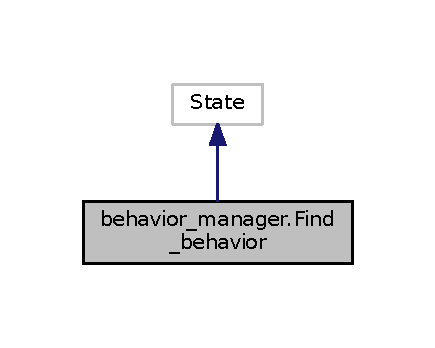
\includegraphics[width=209pt]{classbehavior__manager_1_1Find__behavior__inherit__graph}
\end{center}
\end{figure}


Collaboration diagram for behavior\+\_\+manager.\+Find\+\_\+behavior\+:
\nopagebreak
\begin{figure}[H]
\begin{center}
\leavevmode
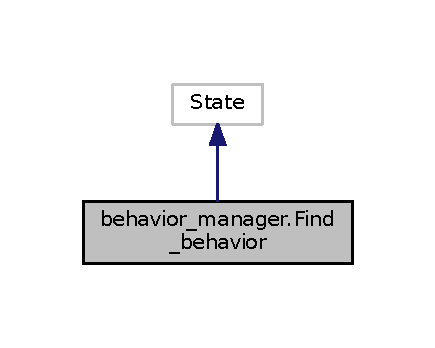
\includegraphics[width=209pt]{classbehavior__manager_1_1Find__behavior__coll__graph}
\end{center}
\end{figure}
\subsection*{Public Member Functions}
\begin{DoxyCompactItemize}
\item 
def \hyperlink{classbehavior__manager_1_1Find__behavior_a38692d816780c602e287a4331cb99a98}{\+\_\+\+\_\+init\+\_\+\+\_\+} (self)
\begin{DoxyCompactList}\small\item\em method init \end{DoxyCompactList}\item 
def \hyperlink{classbehavior__manager_1_1Find__behavior_af12b4ba2e8206c80f55f147c9eb58dc2}{execute} (self, userdata)
\begin{DoxyCompactList}\small\item\em method execute \end{DoxyCompactList}\item 
def \hyperlink{classbehavior__manager_1_1Find__behavior_a092d9fc8598a11ea31c47f07b01e984c}{ball\+\_\+tracking} (self, ball)
\begin{DoxyCompactList}\small\item\em method ball\+\_\+tracking \end{DoxyCompactList}\end{DoxyCompactItemize}
\subsection*{Public Attributes}
\begin{DoxyCompactItemize}
\item 
\hyperlink{classbehavior__manager_1_1Find__behavior_a3671a945907edc316dcc8dd00a219268}{rate}
\item 
\hyperlink{classbehavior__manager_1_1Find__behavior_a45d5bea7497f4a68cf3feb3ba6eb2b19}{movebase\+Client}
\item 
\hyperlink{classbehavior__manager_1_1Find__behavior_aa36ffbc4705c25c0ec23ff688f72b46f}{ball\+\_\+visible}
\end{DoxyCompactItemize}


\subsection{Detailed Description}
class \hyperlink{classbehavior__manager_1_1Find__behavior}{Find\+\_\+behavior} 

when entering Find behaviour, the robot moves randomly within the environment once it detect a coloured ball, it enters the substate Find Track 

\subsection{Constructor \& Destructor Documentation}
\index{behavior\+\_\+manager\+::\+Find\+\_\+behavior@{behavior\+\_\+manager\+::\+Find\+\_\+behavior}!\+\_\+\+\_\+init\+\_\+\+\_\+@{\+\_\+\+\_\+init\+\_\+\+\_\+}}
\index{\+\_\+\+\_\+init\+\_\+\+\_\+@{\+\_\+\+\_\+init\+\_\+\+\_\+}!behavior\+\_\+manager\+::\+Find\+\_\+behavior@{behavior\+\_\+manager\+::\+Find\+\_\+behavior}}
\subsubsection[{\texorpdfstring{\+\_\+\+\_\+init\+\_\+\+\_\+(self)}{__init__(self)}}]{\setlength{\rightskip}{0pt plus 5cm}def behavior\+\_\+manager.\+Find\+\_\+behavior.\+\_\+\+\_\+init\+\_\+\+\_\+ (
\begin{DoxyParamCaption}
\item[{}]{self}
\end{DoxyParamCaption}
)}\hypertarget{classbehavior__manager_1_1Find__behavior_a38692d816780c602e287a4331cb99a98}{}\label{classbehavior__manager_1_1Find__behavior_a38692d816780c602e287a4331cb99a98}


method init 

initialization 

\subsection{Member Function Documentation}
\index{behavior\+\_\+manager\+::\+Find\+\_\+behavior@{behavior\+\_\+manager\+::\+Find\+\_\+behavior}!ball\+\_\+tracking@{ball\+\_\+tracking}}
\index{ball\+\_\+tracking@{ball\+\_\+tracking}!behavior\+\_\+manager\+::\+Find\+\_\+behavior@{behavior\+\_\+manager\+::\+Find\+\_\+behavior}}
\subsubsection[{\texorpdfstring{ball\+\_\+tracking(self, ball)}{ball_tracking(self, ball)}}]{\setlength{\rightskip}{0pt plus 5cm}def behavior\+\_\+manager.\+Find\+\_\+behavior.\+ball\+\_\+tracking (
\begin{DoxyParamCaption}
\item[{}]{self, }
\item[{}]{ball}
\end{DoxyParamCaption}
)}\hypertarget{classbehavior__manager_1_1Find__behavior_a092d9fc8598a11ea31c47f07b01e984c}{}\label{classbehavior__manager_1_1Find__behavior_a092d9fc8598a11ea31c47f07b01e984c}


method ball\+\_\+tracking 

subscriber call \index{behavior\+\_\+manager\+::\+Find\+\_\+behavior@{behavior\+\_\+manager\+::\+Find\+\_\+behavior}!execute@{execute}}
\index{execute@{execute}!behavior\+\_\+manager\+::\+Find\+\_\+behavior@{behavior\+\_\+manager\+::\+Find\+\_\+behavior}}
\subsubsection[{\texorpdfstring{execute(self, userdata)}{execute(self, userdata)}}]{\setlength{\rightskip}{0pt plus 5cm}def behavior\+\_\+manager.\+Find\+\_\+behavior.\+execute (
\begin{DoxyParamCaption}
\item[{}]{self, }
\item[{}]{userdata}
\end{DoxyParamCaption}
)}\hypertarget{classbehavior__manager_1_1Find__behavior_af12b4ba2e8206c80f55f147c9eb58dc2}{}\label{classbehavior__manager_1_1Find__behavior_af12b4ba2e8206c80f55f147c9eb58dc2}


method execute 

state execution 

\subsection{Member Data Documentation}
\index{behavior\+\_\+manager\+::\+Find\+\_\+behavior@{behavior\+\_\+manager\+::\+Find\+\_\+behavior}!ball\+\_\+visible@{ball\+\_\+visible}}
\index{ball\+\_\+visible@{ball\+\_\+visible}!behavior\+\_\+manager\+::\+Find\+\_\+behavior@{behavior\+\_\+manager\+::\+Find\+\_\+behavior}}
\subsubsection[{\texorpdfstring{ball\+\_\+visible}{ball_visible}}]{\setlength{\rightskip}{0pt plus 5cm}behavior\+\_\+manager.\+Find\+\_\+behavior.\+ball\+\_\+visible}\hypertarget{classbehavior__manager_1_1Find__behavior_aa36ffbc4705c25c0ec23ff688f72b46f}{}\label{classbehavior__manager_1_1Find__behavior_aa36ffbc4705c25c0ec23ff688f72b46f}
\index{behavior\+\_\+manager\+::\+Find\+\_\+behavior@{behavior\+\_\+manager\+::\+Find\+\_\+behavior}!movebase\+Client@{movebase\+Client}}
\index{movebase\+Client@{movebase\+Client}!behavior\+\_\+manager\+::\+Find\+\_\+behavior@{behavior\+\_\+manager\+::\+Find\+\_\+behavior}}
\subsubsection[{\texorpdfstring{movebase\+Client}{movebaseClient}}]{\setlength{\rightskip}{0pt plus 5cm}behavior\+\_\+manager.\+Find\+\_\+behavior.\+movebase\+Client}\hypertarget{classbehavior__manager_1_1Find__behavior_a45d5bea7497f4a68cf3feb3ba6eb2b19}{}\label{classbehavior__manager_1_1Find__behavior_a45d5bea7497f4a68cf3feb3ba6eb2b19}
\index{behavior\+\_\+manager\+::\+Find\+\_\+behavior@{behavior\+\_\+manager\+::\+Find\+\_\+behavior}!rate@{rate}}
\index{rate@{rate}!behavior\+\_\+manager\+::\+Find\+\_\+behavior@{behavior\+\_\+manager\+::\+Find\+\_\+behavior}}
\subsubsection[{\texorpdfstring{rate}{rate}}]{\setlength{\rightskip}{0pt plus 5cm}behavior\+\_\+manager.\+Find\+\_\+behavior.\+rate}\hypertarget{classbehavior__manager_1_1Find__behavior_a3671a945907edc316dcc8dd00a219268}{}\label{classbehavior__manager_1_1Find__behavior_a3671a945907edc316dcc8dd00a219268}


The documentation for this class was generated from the following file\+:\begin{DoxyCompactItemize}
\item 
/home/\+Experimental\+Robotics\+Lab\+Serena/src/exp\+\_\+assignment3/src/\hyperlink{behavior__manager_8py}{behavior\+\_\+manager.\+py}\end{DoxyCompactItemize}

\hypertarget{classbehavior__manager_1_1Find__track__behaviour}{}\section{behavior\+\_\+manager.\+Find\+\_\+track\+\_\+behaviour Class Reference}
\label{classbehavior__manager_1_1Find__track__behaviour}\index{behavior\+\_\+manager.\+Find\+\_\+track\+\_\+behaviour@{behavior\+\_\+manager.\+Find\+\_\+track\+\_\+behaviour}}


class \hyperlink{classbehavior__manager_1_1Find__track__behaviour}{Find\+\_\+track\+\_\+behaviour}  




Inheritance diagram for behavior\+\_\+manager.\+Find\+\_\+track\+\_\+behaviour\+:
\nopagebreak
\begin{figure}[H]
\begin{center}
\leavevmode
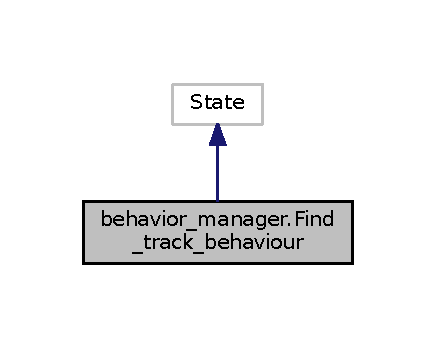
\includegraphics[width=209pt]{classbehavior__manager_1_1Find__track__behaviour__inherit__graph}
\end{center}
\end{figure}


Collaboration diagram for behavior\+\_\+manager.\+Find\+\_\+track\+\_\+behaviour\+:
\nopagebreak
\begin{figure}[H]
\begin{center}
\leavevmode
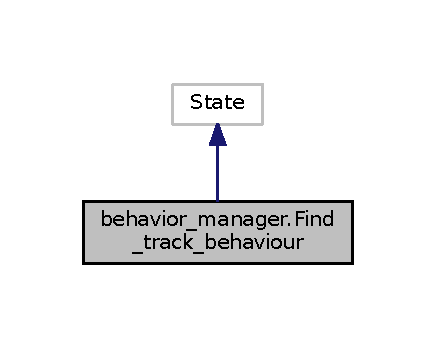
\includegraphics[width=209pt]{classbehavior__manager_1_1Find__track__behaviour__coll__graph}
\end{center}
\end{figure}
\subsection*{Public Member Functions}
\begin{DoxyCompactItemize}
\item 
def \hyperlink{classbehavior__manager_1_1Find__track__behaviour_a1c9e21684b80b7c55250e5c51db162ef}{\+\_\+\+\_\+init\+\_\+\+\_\+} (self)
\begin{DoxyCompactList}\small\item\em method init \end{DoxyCompactList}\item 
def \hyperlink{classbehavior__manager_1_1Find__track__behaviour_abc08716d3814807c7e310a1726b1f0d2}{execute} (self, userdata)
\begin{DoxyCompactList}\small\item\em method execute \end{DoxyCompactList}\item 
def \hyperlink{classbehavior__manager_1_1Find__track__behaviour_a07860df69cff5dfcd0f0e1d06127b831}{check\+\_\+at\+\_\+ball} (self, ball)
\begin{DoxyCompactList}\small\item\em method check\+\_\+at\+\_\+ball \end{DoxyCompactList}\item 
def \hyperlink{classbehavior__manager_1_1Find__track__behaviour_a6d00b24d466d797df6db40960c8117c3}{check\+\_\+at\+\_\+room} (self, room)
\begin{DoxyCompactList}\small\item\em method check\+\_\+at\+\_\+room \end{DoxyCompactList}\end{DoxyCompactItemize}
\subsection*{Public Attributes}
\begin{DoxyCompactItemize}
\item 
\hyperlink{classbehavior__manager_1_1Find__track__behaviour_a2f4d1da1a2f987c83f65f22ecdf52735}{rate}
\item 
\hyperlink{classbehavior__manager_1_1Find__track__behaviour_a6e7788d035404b0eaf79ad5e03fcb697}{at\+\_\+ball}
\item 
\hyperlink{classbehavior__manager_1_1Find__track__behaviour_a88ccf669e65adb99390ee8690b7b7b47}{at\+\_\+room}
\end{DoxyCompactItemize}


\subsection{Detailed Description}
class \hyperlink{classbehavior__manager_1_1Find__track__behaviour}{Find\+\_\+track\+\_\+behaviour} 

substate of the robot from Find behaviour 

\subsection{Constructor \& Destructor Documentation}
\index{behavior\+\_\+manager\+::\+Find\+\_\+track\+\_\+behaviour@{behavior\+\_\+manager\+::\+Find\+\_\+track\+\_\+behaviour}!\+\_\+\+\_\+init\+\_\+\+\_\+@{\+\_\+\+\_\+init\+\_\+\+\_\+}}
\index{\+\_\+\+\_\+init\+\_\+\+\_\+@{\+\_\+\+\_\+init\+\_\+\+\_\+}!behavior\+\_\+manager\+::\+Find\+\_\+track\+\_\+behaviour@{behavior\+\_\+manager\+::\+Find\+\_\+track\+\_\+behaviour}}
\subsubsection[{\texorpdfstring{\+\_\+\+\_\+init\+\_\+\+\_\+(self)}{__init__(self)}}]{\setlength{\rightskip}{0pt plus 5cm}def behavior\+\_\+manager.\+Find\+\_\+track\+\_\+behaviour.\+\_\+\+\_\+init\+\_\+\+\_\+ (
\begin{DoxyParamCaption}
\item[{}]{self}
\end{DoxyParamCaption}
)}\hypertarget{classbehavior__manager_1_1Find__track__behaviour_a1c9e21684b80b7c55250e5c51db162ef}{}\label{classbehavior__manager_1_1Find__track__behaviour_a1c9e21684b80b7c55250e5c51db162ef}


method init 

initialization 

\subsection{Member Function Documentation}
\index{behavior\+\_\+manager\+::\+Find\+\_\+track\+\_\+behaviour@{behavior\+\_\+manager\+::\+Find\+\_\+track\+\_\+behaviour}!check\+\_\+at\+\_\+ball@{check\+\_\+at\+\_\+ball}}
\index{check\+\_\+at\+\_\+ball@{check\+\_\+at\+\_\+ball}!behavior\+\_\+manager\+::\+Find\+\_\+track\+\_\+behaviour@{behavior\+\_\+manager\+::\+Find\+\_\+track\+\_\+behaviour}}
\subsubsection[{\texorpdfstring{check\+\_\+at\+\_\+ball(self, ball)}{check_at_ball(self, ball)}}]{\setlength{\rightskip}{0pt plus 5cm}def behavior\+\_\+manager.\+Find\+\_\+track\+\_\+behaviour.\+check\+\_\+at\+\_\+ball (
\begin{DoxyParamCaption}
\item[{}]{self, }
\item[{}]{ball}
\end{DoxyParamCaption}
)}\hypertarget{classbehavior__manager_1_1Find__track__behaviour_a07860df69cff5dfcd0f0e1d06127b831}{}\label{classbehavior__manager_1_1Find__track__behaviour_a07860df69cff5dfcd0f0e1d06127b831}


method check\+\_\+at\+\_\+ball 

callback to check if the robot is close at the detected ball \index{behavior\+\_\+manager\+::\+Find\+\_\+track\+\_\+behaviour@{behavior\+\_\+manager\+::\+Find\+\_\+track\+\_\+behaviour}!check\+\_\+at\+\_\+room@{check\+\_\+at\+\_\+room}}
\index{check\+\_\+at\+\_\+room@{check\+\_\+at\+\_\+room}!behavior\+\_\+manager\+::\+Find\+\_\+track\+\_\+behaviour@{behavior\+\_\+manager\+::\+Find\+\_\+track\+\_\+behaviour}}
\subsubsection[{\texorpdfstring{check\+\_\+at\+\_\+room(self, room)}{check_at_room(self, room)}}]{\setlength{\rightskip}{0pt plus 5cm}def behavior\+\_\+manager.\+Find\+\_\+track\+\_\+behaviour.\+check\+\_\+at\+\_\+room (
\begin{DoxyParamCaption}
\item[{}]{self, }
\item[{}]{room}
\end{DoxyParamCaption}
)}\hypertarget{classbehavior__manager_1_1Find__track__behaviour_a6d00b24d466d797df6db40960c8117c3}{}\label{classbehavior__manager_1_1Find__track__behaviour_a6d00b24d466d797df6db40960c8117c3}


method check\+\_\+at\+\_\+room 

callback to check if the robot is close at the detected ball \index{behavior\+\_\+manager\+::\+Find\+\_\+track\+\_\+behaviour@{behavior\+\_\+manager\+::\+Find\+\_\+track\+\_\+behaviour}!execute@{execute}}
\index{execute@{execute}!behavior\+\_\+manager\+::\+Find\+\_\+track\+\_\+behaviour@{behavior\+\_\+manager\+::\+Find\+\_\+track\+\_\+behaviour}}
\subsubsection[{\texorpdfstring{execute(self, userdata)}{execute(self, userdata)}}]{\setlength{\rightskip}{0pt plus 5cm}def behavior\+\_\+manager.\+Find\+\_\+track\+\_\+behaviour.\+execute (
\begin{DoxyParamCaption}
\item[{}]{self, }
\item[{}]{userdata}
\end{DoxyParamCaption}
)}\hypertarget{classbehavior__manager_1_1Find__track__behaviour_abc08716d3814807c7e310a1726b1f0d2}{}\label{classbehavior__manager_1_1Find__track__behaviour_abc08716d3814807c7e310a1726b1f0d2}


method execute 

state execution 

\subsection{Member Data Documentation}
\index{behavior\+\_\+manager\+::\+Find\+\_\+track\+\_\+behaviour@{behavior\+\_\+manager\+::\+Find\+\_\+track\+\_\+behaviour}!at\+\_\+ball@{at\+\_\+ball}}
\index{at\+\_\+ball@{at\+\_\+ball}!behavior\+\_\+manager\+::\+Find\+\_\+track\+\_\+behaviour@{behavior\+\_\+manager\+::\+Find\+\_\+track\+\_\+behaviour}}
\subsubsection[{\texorpdfstring{at\+\_\+ball}{at_ball}}]{\setlength{\rightskip}{0pt plus 5cm}behavior\+\_\+manager.\+Find\+\_\+track\+\_\+behaviour.\+at\+\_\+ball}\hypertarget{classbehavior__manager_1_1Find__track__behaviour_a6e7788d035404b0eaf79ad5e03fcb697}{}\label{classbehavior__manager_1_1Find__track__behaviour_a6e7788d035404b0eaf79ad5e03fcb697}
\index{behavior\+\_\+manager\+::\+Find\+\_\+track\+\_\+behaviour@{behavior\+\_\+manager\+::\+Find\+\_\+track\+\_\+behaviour}!at\+\_\+room@{at\+\_\+room}}
\index{at\+\_\+room@{at\+\_\+room}!behavior\+\_\+manager\+::\+Find\+\_\+track\+\_\+behaviour@{behavior\+\_\+manager\+::\+Find\+\_\+track\+\_\+behaviour}}
\subsubsection[{\texorpdfstring{at\+\_\+room}{at_room}}]{\setlength{\rightskip}{0pt plus 5cm}behavior\+\_\+manager.\+Find\+\_\+track\+\_\+behaviour.\+at\+\_\+room}\hypertarget{classbehavior__manager_1_1Find__track__behaviour_a88ccf669e65adb99390ee8690b7b7b47}{}\label{classbehavior__manager_1_1Find__track__behaviour_a88ccf669e65adb99390ee8690b7b7b47}
\index{behavior\+\_\+manager\+::\+Find\+\_\+track\+\_\+behaviour@{behavior\+\_\+manager\+::\+Find\+\_\+track\+\_\+behaviour}!rate@{rate}}
\index{rate@{rate}!behavior\+\_\+manager\+::\+Find\+\_\+track\+\_\+behaviour@{behavior\+\_\+manager\+::\+Find\+\_\+track\+\_\+behaviour}}
\subsubsection[{\texorpdfstring{rate}{rate}}]{\setlength{\rightskip}{0pt plus 5cm}behavior\+\_\+manager.\+Find\+\_\+track\+\_\+behaviour.\+rate}\hypertarget{classbehavior__manager_1_1Find__track__behaviour_a2f4d1da1a2f987c83f65f22ecdf52735}{}\label{classbehavior__manager_1_1Find__track__behaviour_a2f4d1da1a2f987c83f65f22ecdf52735}


The documentation for this class was generated from the following file\+:\begin{DoxyCompactItemize}
\item 
/home/\+Experimental\+Robotics\+Lab\+Serena/src/exp\+\_\+assignment3/src/\hyperlink{behavior__manager_8py}{behavior\+\_\+manager.\+py}\end{DoxyCompactItemize}

\hypertarget{classbehavior__manager_1_1Normal__behavior}{}\section{behavior\+\_\+manager.\+Normal\+\_\+behavior Class Reference}
\label{classbehavior__manager_1_1Normal__behavior}\index{behavior\+\_\+manager.\+Normal\+\_\+behavior@{behavior\+\_\+manager.\+Normal\+\_\+behavior}}


class \hyperlink{classbehavior__manager_1_1Normal__behavior}{Normal\+\_\+behavior}  




Inheritance diagram for behavior\+\_\+manager.\+Normal\+\_\+behavior\+:
\nopagebreak
\begin{figure}[H]
\begin{center}
\leavevmode
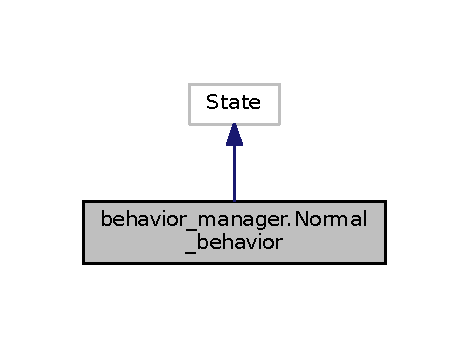
\includegraphics[width=225pt]{classbehavior__manager_1_1Normal__behavior__inherit__graph}
\end{center}
\end{figure}


Collaboration diagram for behavior\+\_\+manager.\+Normal\+\_\+behavior\+:
\nopagebreak
\begin{figure}[H]
\begin{center}
\leavevmode
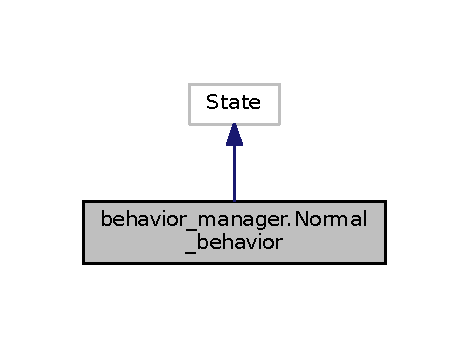
\includegraphics[width=225pt]{classbehavior__manager_1_1Normal__behavior__coll__graph}
\end{center}
\end{figure}
\subsection*{Public Member Functions}
\begin{DoxyCompactItemize}
\item 
def \hyperlink{classbehavior__manager_1_1Normal__behavior_a7ab22900e936fc3921a269389b51e6ab}{\+\_\+\+\_\+init\+\_\+\+\_\+} (self)
\begin{DoxyCompactList}\small\item\em method init \end{DoxyCompactList}\item 
def \hyperlink{classbehavior__manager_1_1Normal__behavior_a15faab6a43a39510355baad4faaa808a}{execute} (self, userdata)
\begin{DoxyCompactList}\small\item\em method execute \end{DoxyCompactList}\item 
def \hyperlink{classbehavior__manager_1_1Normal__behavior_a19d07d077327e725321bc7d13aa3726e}{ball\+\_\+tracking} (self, ball)
\begin{DoxyCompactList}\small\item\em method ball\+\_\+tracking \end{DoxyCompactList}\item 
def \hyperlink{classbehavior__manager_1_1Normal__behavior_a5a152cc5837f1573c5101f18e86d7070}{read\+\_\+command} (self, human\+\_\+command)
\begin{DoxyCompactList}\small\item\em method read\+\_\+command \end{DoxyCompactList}\end{DoxyCompactItemize}
\subsection*{Public Attributes}
\begin{DoxyCompactItemize}
\item 
\hyperlink{classbehavior__manager_1_1Normal__behavior_a8c0881c34370caec4f5298f0ebe35489}{rate}
\item 
\hyperlink{classbehavior__manager_1_1Normal__behavior_ad3ddfca519e8fa6513d6356aa0fa2962}{human\+\_\+command\+\_\+play}
\item 
\hyperlink{classbehavior__manager_1_1Normal__behavior_a9231755f61898994c43ae8e5652ef1c9}{ball\+\_\+visible}
\end{DoxyCompactItemize}


\subsection{Detailed Description}
class \hyperlink{classbehavior__manager_1_1Normal__behavior}{Normal\+\_\+behavior} 

This class implement the N\+O\+R\+M\+AL behaviour of the robot pet The robot moves randomly within the Gazebo arena
\begin{DoxyItemize}
\item If it receives a \char`\"{}play\char`\"{} command the F\+SM should go into P\+L\+AY state (start\+\_\+play)
\item If the sleep timer is triggered the F\+SM should go into S\+L\+E\+EP state (start\+\_\+sleep) 
\end{DoxyItemize}

\subsection{Constructor \& Destructor Documentation}
\index{behavior\+\_\+manager\+::\+Normal\+\_\+behavior@{behavior\+\_\+manager\+::\+Normal\+\_\+behavior}!\+\_\+\+\_\+init\+\_\+\+\_\+@{\+\_\+\+\_\+init\+\_\+\+\_\+}}
\index{\+\_\+\+\_\+init\+\_\+\+\_\+@{\+\_\+\+\_\+init\+\_\+\+\_\+}!behavior\+\_\+manager\+::\+Normal\+\_\+behavior@{behavior\+\_\+manager\+::\+Normal\+\_\+behavior}}
\subsubsection[{\texorpdfstring{\+\_\+\+\_\+init\+\_\+\+\_\+(self)}{__init__(self)}}]{\setlength{\rightskip}{0pt plus 5cm}def behavior\+\_\+manager.\+Normal\+\_\+behavior.\+\_\+\+\_\+init\+\_\+\+\_\+ (
\begin{DoxyParamCaption}
\item[{}]{self}
\end{DoxyParamCaption}
)}\hypertarget{classbehavior__manager_1_1Normal__behavior_a7ab22900e936fc3921a269389b51e6ab}{}\label{classbehavior__manager_1_1Normal__behavior_a7ab22900e936fc3921a269389b51e6ab}


method init 

This method should\+:
\begin{DoxyItemize}
\item initializes the state class 
\end{DoxyItemize}

\subsection{Member Function Documentation}
\index{behavior\+\_\+manager\+::\+Normal\+\_\+behavior@{behavior\+\_\+manager\+::\+Normal\+\_\+behavior}!ball\+\_\+tracking@{ball\+\_\+tracking}}
\index{ball\+\_\+tracking@{ball\+\_\+tracking}!behavior\+\_\+manager\+::\+Normal\+\_\+behavior@{behavior\+\_\+manager\+::\+Normal\+\_\+behavior}}
\subsubsection[{\texorpdfstring{ball\+\_\+tracking(self, ball)}{ball_tracking(self, ball)}}]{\setlength{\rightskip}{0pt plus 5cm}def behavior\+\_\+manager.\+Normal\+\_\+behavior.\+ball\+\_\+tracking (
\begin{DoxyParamCaption}
\item[{}]{self, }
\item[{}]{ball}
\end{DoxyParamCaption}
)}\hypertarget{classbehavior__manager_1_1Normal__behavior_a19d07d077327e725321bc7d13aa3726e}{}\label{classbehavior__manager_1_1Normal__behavior_a19d07d077327e725321bc7d13aa3726e}


method ball\+\_\+tracking 

method to check if the ball is visible to the robot or not \index{behavior\+\_\+manager\+::\+Normal\+\_\+behavior@{behavior\+\_\+manager\+::\+Normal\+\_\+behavior}!execute@{execute}}
\index{execute@{execute}!behavior\+\_\+manager\+::\+Normal\+\_\+behavior@{behavior\+\_\+manager\+::\+Normal\+\_\+behavior}}
\subsubsection[{\texorpdfstring{execute(self, userdata)}{execute(self, userdata)}}]{\setlength{\rightskip}{0pt plus 5cm}def behavior\+\_\+manager.\+Normal\+\_\+behavior.\+execute (
\begin{DoxyParamCaption}
\item[{}]{self, }
\item[{}]{userdata}
\end{DoxyParamCaption}
)}\hypertarget{classbehavior__manager_1_1Normal__behavior_a15faab6a43a39510355baad4faaa808a}{}\label{classbehavior__manager_1_1Normal__behavior_a15faab6a43a39510355baad4faaa808a}


method execute 


\begin{DoxyItemize}
\item publish \char`\"{}normal\char`\"{} (String) on the topic behavior
\item moves the robot randomly
\item if a command from the human is received
\begin{DoxyItemize}
\item the robot switches to Play state
\end{DoxyItemize}
\item if the ball is visible\+:
\begin{DoxyItemize}
\item the robot switches to Normal Track sub state 
\end{DoxyItemize}
\end{DoxyItemize}\index{behavior\+\_\+manager\+::\+Normal\+\_\+behavior@{behavior\+\_\+manager\+::\+Normal\+\_\+behavior}!read\+\_\+command@{read\+\_\+command}}
\index{read\+\_\+command@{read\+\_\+command}!behavior\+\_\+manager\+::\+Normal\+\_\+behavior@{behavior\+\_\+manager\+::\+Normal\+\_\+behavior}}
\subsubsection[{\texorpdfstring{read\+\_\+command(self, human\+\_\+command)}{read_command(self, human_command)}}]{\setlength{\rightskip}{0pt plus 5cm}def behavior\+\_\+manager.\+Normal\+\_\+behavior.\+read\+\_\+command (
\begin{DoxyParamCaption}
\item[{}]{self, }
\item[{}]{human\+\_\+command}
\end{DoxyParamCaption}
)}\hypertarget{classbehavior__manager_1_1Normal__behavior_a5a152cc5837f1573c5101f18e86d7070}{}\label{classbehavior__manager_1_1Normal__behavior_a5a152cc5837f1573c5101f18e86d7070}


method read\+\_\+command 

method to check if if received a command or not 

\subsection{Member Data Documentation}
\index{behavior\+\_\+manager\+::\+Normal\+\_\+behavior@{behavior\+\_\+manager\+::\+Normal\+\_\+behavior}!ball\+\_\+visible@{ball\+\_\+visible}}
\index{ball\+\_\+visible@{ball\+\_\+visible}!behavior\+\_\+manager\+::\+Normal\+\_\+behavior@{behavior\+\_\+manager\+::\+Normal\+\_\+behavior}}
\subsubsection[{\texorpdfstring{ball\+\_\+visible}{ball_visible}}]{\setlength{\rightskip}{0pt plus 5cm}behavior\+\_\+manager.\+Normal\+\_\+behavior.\+ball\+\_\+visible}\hypertarget{classbehavior__manager_1_1Normal__behavior_a9231755f61898994c43ae8e5652ef1c9}{}\label{classbehavior__manager_1_1Normal__behavior_a9231755f61898994c43ae8e5652ef1c9}
\index{behavior\+\_\+manager\+::\+Normal\+\_\+behavior@{behavior\+\_\+manager\+::\+Normal\+\_\+behavior}!human\+\_\+command\+\_\+play@{human\+\_\+command\+\_\+play}}
\index{human\+\_\+command\+\_\+play@{human\+\_\+command\+\_\+play}!behavior\+\_\+manager\+::\+Normal\+\_\+behavior@{behavior\+\_\+manager\+::\+Normal\+\_\+behavior}}
\subsubsection[{\texorpdfstring{human\+\_\+command\+\_\+play}{human_command_play}}]{\setlength{\rightskip}{0pt plus 5cm}behavior\+\_\+manager.\+Normal\+\_\+behavior.\+human\+\_\+command\+\_\+play}\hypertarget{classbehavior__manager_1_1Normal__behavior_ad3ddfca519e8fa6513d6356aa0fa2962}{}\label{classbehavior__manager_1_1Normal__behavior_ad3ddfca519e8fa6513d6356aa0fa2962}
\index{behavior\+\_\+manager\+::\+Normal\+\_\+behavior@{behavior\+\_\+manager\+::\+Normal\+\_\+behavior}!rate@{rate}}
\index{rate@{rate}!behavior\+\_\+manager\+::\+Normal\+\_\+behavior@{behavior\+\_\+manager\+::\+Normal\+\_\+behavior}}
\subsubsection[{\texorpdfstring{rate}{rate}}]{\setlength{\rightskip}{0pt plus 5cm}behavior\+\_\+manager.\+Normal\+\_\+behavior.\+rate}\hypertarget{classbehavior__manager_1_1Normal__behavior_a8c0881c34370caec4f5298f0ebe35489}{}\label{classbehavior__manager_1_1Normal__behavior_a8c0881c34370caec4f5298f0ebe35489}


The documentation for this class was generated from the following file\+:\begin{DoxyCompactItemize}
\item 
/home/\+Experimental\+Robotics\+Lab\+Serena/src/exp\+\_\+assignment3/src/\hyperlink{behavior__manager_8py}{behavior\+\_\+manager.\+py}\end{DoxyCompactItemize}

\hypertarget{classbehavior__manager_1_1Normal__track__behaviour}{}\section{behavior\+\_\+manager.\+Normal\+\_\+track\+\_\+behaviour Class Reference}
\label{classbehavior__manager_1_1Normal__track__behaviour}\index{behavior\+\_\+manager.\+Normal\+\_\+track\+\_\+behaviour@{behavior\+\_\+manager.\+Normal\+\_\+track\+\_\+behaviour}}


class \hyperlink{classbehavior__manager_1_1Normal__track__behaviour}{Normal\+\_\+track\+\_\+behaviour}  




Inheritance diagram for behavior\+\_\+manager.\+Normal\+\_\+track\+\_\+behaviour\+:
\nopagebreak
\begin{figure}[H]
\begin{center}
\leavevmode
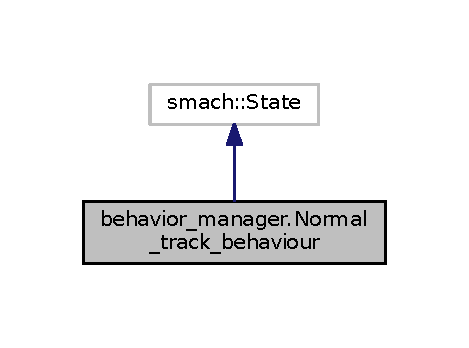
\includegraphics[width=225pt]{classbehavior__manager_1_1Normal__track__behaviour__inherit__graph}
\end{center}
\end{figure}


Collaboration diagram for behavior\+\_\+manager.\+Normal\+\_\+track\+\_\+behaviour\+:
\nopagebreak
\begin{figure}[H]
\begin{center}
\leavevmode
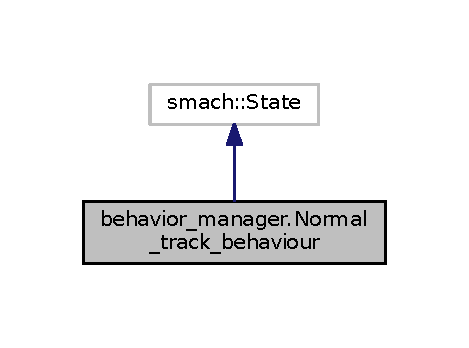
\includegraphics[width=225pt]{classbehavior__manager_1_1Normal__track__behaviour__coll__graph}
\end{center}
\end{figure}
\subsection*{Public Member Functions}
\begin{DoxyCompactItemize}
\item 
def \hyperlink{classbehavior__manager_1_1Normal__track__behaviour_ad442bd3a8b510459e8271075e1e7f8f1}{\+\_\+\+\_\+init\+\_\+\+\_\+} (self)
\begin{DoxyCompactList}\small\item\em method init \end{DoxyCompactList}\item 
def \hyperlink{classbehavior__manager_1_1Normal__track__behaviour_a3bbad6b9c6733364eacf193d387c2397}{execute} (self, userdata)
\begin{DoxyCompactList}\small\item\em method execute \end{DoxyCompactList}\item 
def \hyperlink{classbehavior__manager_1_1Normal__track__behaviour_a1e37969e88239c54d307769f1bb042ab}{check\+\_\+at\+\_\+ball} (self, check)
\end{DoxyCompactItemize}
\subsection*{Public Attributes}
\begin{DoxyCompactItemize}
\item 
\hyperlink{classbehavior__manager_1_1Normal__track__behaviour_a208545700e8ed6da275c4d706f7c1abd}{rate}
\item 
\hyperlink{classbehavior__manager_1_1Normal__track__behaviour_a1c8562aa75539239ac6dc0ac1b286f84}{at\+\_\+ball}
\end{DoxyCompactItemize}


\subsection{Detailed Description}
class \hyperlink{classbehavior__manager_1_1Normal__track__behaviour}{Normal\+\_\+track\+\_\+behaviour} 

substate of the Normal state. When the robot sees a ball while in Normal state it tries to move closer and store its position 

\subsection{Constructor \& Destructor Documentation}
\index{behavior\+\_\+manager\+::\+Normal\+\_\+track\+\_\+behaviour@{behavior\+\_\+manager\+::\+Normal\+\_\+track\+\_\+behaviour}!\+\_\+\+\_\+init\+\_\+\+\_\+@{\+\_\+\+\_\+init\+\_\+\+\_\+}}
\index{\+\_\+\+\_\+init\+\_\+\+\_\+@{\+\_\+\+\_\+init\+\_\+\+\_\+}!behavior\+\_\+manager\+::\+Normal\+\_\+track\+\_\+behaviour@{behavior\+\_\+manager\+::\+Normal\+\_\+track\+\_\+behaviour}}
\subsubsection[{\texorpdfstring{\+\_\+\+\_\+init\+\_\+\+\_\+(self)}{__init__(self)}}]{\setlength{\rightskip}{0pt plus 5cm}def behavior\+\_\+manager.\+Normal\+\_\+track\+\_\+behaviour.\+\_\+\+\_\+init\+\_\+\+\_\+ (
\begin{DoxyParamCaption}
\item[{}]{self}
\end{DoxyParamCaption}
)}\hypertarget{classbehavior__manager_1_1Normal__track__behaviour_ad442bd3a8b510459e8271075e1e7f8f1}{}\label{classbehavior__manager_1_1Normal__track__behaviour_ad442bd3a8b510459e8271075e1e7f8f1}


method init 

state initialization 

\subsection{Member Function Documentation}
\index{behavior\+\_\+manager\+::\+Normal\+\_\+track\+\_\+behaviour@{behavior\+\_\+manager\+::\+Normal\+\_\+track\+\_\+behaviour}!check\+\_\+at\+\_\+ball@{check\+\_\+at\+\_\+ball}}
\index{check\+\_\+at\+\_\+ball@{check\+\_\+at\+\_\+ball}!behavior\+\_\+manager\+::\+Normal\+\_\+track\+\_\+behaviour@{behavior\+\_\+manager\+::\+Normal\+\_\+track\+\_\+behaviour}}
\subsubsection[{\texorpdfstring{check\+\_\+at\+\_\+ball(self, check)}{check_at_ball(self, check)}}]{\setlength{\rightskip}{0pt plus 5cm}def behavior\+\_\+manager.\+Normal\+\_\+track\+\_\+behaviour.\+check\+\_\+at\+\_\+ball (
\begin{DoxyParamCaption}
\item[{}]{self, }
\item[{}]{check}
\end{DoxyParamCaption}
)}\hypertarget{classbehavior__manager_1_1Normal__track__behaviour_a1e37969e88239c54d307769f1bb042ab}{}\label{classbehavior__manager_1_1Normal__track__behaviour_a1e37969e88239c54d307769f1bb042ab}
\index{behavior\+\_\+manager\+::\+Normal\+\_\+track\+\_\+behaviour@{behavior\+\_\+manager\+::\+Normal\+\_\+track\+\_\+behaviour}!execute@{execute}}
\index{execute@{execute}!behavior\+\_\+manager\+::\+Normal\+\_\+track\+\_\+behaviour@{behavior\+\_\+manager\+::\+Normal\+\_\+track\+\_\+behaviour}}
\subsubsection[{\texorpdfstring{execute(self, userdata)}{execute(self, userdata)}}]{\setlength{\rightskip}{0pt plus 5cm}def behavior\+\_\+manager.\+Normal\+\_\+track\+\_\+behaviour.\+execute (
\begin{DoxyParamCaption}
\item[{}]{self, }
\item[{}]{userdata}
\end{DoxyParamCaption}
)}\hypertarget{classbehavior__manager_1_1Normal__track__behaviour_a3bbad6b9c6733364eacf193d387c2397}{}\label{classbehavior__manager_1_1Normal__track__behaviour_a3bbad6b9c6733364eacf193d387c2397}


method execute 

once the robot has moved closer to the ball, the function check if it is really close to the ball or not 

\subsection{Member Data Documentation}
\index{behavior\+\_\+manager\+::\+Normal\+\_\+track\+\_\+behaviour@{behavior\+\_\+manager\+::\+Normal\+\_\+track\+\_\+behaviour}!at\+\_\+ball@{at\+\_\+ball}}
\index{at\+\_\+ball@{at\+\_\+ball}!behavior\+\_\+manager\+::\+Normal\+\_\+track\+\_\+behaviour@{behavior\+\_\+manager\+::\+Normal\+\_\+track\+\_\+behaviour}}
\subsubsection[{\texorpdfstring{at\+\_\+ball}{at_ball}}]{\setlength{\rightskip}{0pt plus 5cm}behavior\+\_\+manager.\+Normal\+\_\+track\+\_\+behaviour.\+at\+\_\+ball}\hypertarget{classbehavior__manager_1_1Normal__track__behaviour_a1c8562aa75539239ac6dc0ac1b286f84}{}\label{classbehavior__manager_1_1Normal__track__behaviour_a1c8562aa75539239ac6dc0ac1b286f84}
\index{behavior\+\_\+manager\+::\+Normal\+\_\+track\+\_\+behaviour@{behavior\+\_\+manager\+::\+Normal\+\_\+track\+\_\+behaviour}!rate@{rate}}
\index{rate@{rate}!behavior\+\_\+manager\+::\+Normal\+\_\+track\+\_\+behaviour@{behavior\+\_\+manager\+::\+Normal\+\_\+track\+\_\+behaviour}}
\subsubsection[{\texorpdfstring{rate}{rate}}]{\setlength{\rightskip}{0pt plus 5cm}behavior\+\_\+manager.\+Normal\+\_\+track\+\_\+behaviour.\+rate}\hypertarget{classbehavior__manager_1_1Normal__track__behaviour_a208545700e8ed6da275c4d706f7c1abd}{}\label{classbehavior__manager_1_1Normal__track__behaviour_a208545700e8ed6da275c4d706f7c1abd}


The documentation for this class was generated from the following file\+:\begin{DoxyCompactItemize}
\item 
/home/\+Experimental\+Robotics\+Lab\+Serena/src/exp\+\_\+assignment3/src/\hyperlink{behavior__manager_8py}{behavior\+\_\+manager.\+py}\end{DoxyCompactItemize}

\hypertarget{classbehavior__manager_1_1Play__behavior}{}\section{behavior\+\_\+manager.\+Play\+\_\+behavior Class Reference}
\label{classbehavior__manager_1_1Play__behavior}\index{behavior\+\_\+manager.\+Play\+\_\+behavior@{behavior\+\_\+manager.\+Play\+\_\+behavior}}


class \hyperlink{classbehavior__manager_1_1Play__behavior}{Play\+\_\+behavior}  




Inheritance diagram for behavior\+\_\+manager.\+Play\+\_\+behavior\+:
\nopagebreak
\begin{figure}[H]
\begin{center}
\leavevmode
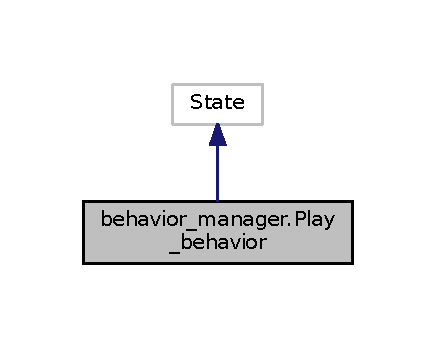
\includegraphics[width=209pt]{classbehavior__manager_1_1Play__behavior__inherit__graph}
\end{center}
\end{figure}


Collaboration diagram for behavior\+\_\+manager.\+Play\+\_\+behavior\+:
\nopagebreak
\begin{figure}[H]
\begin{center}
\leavevmode
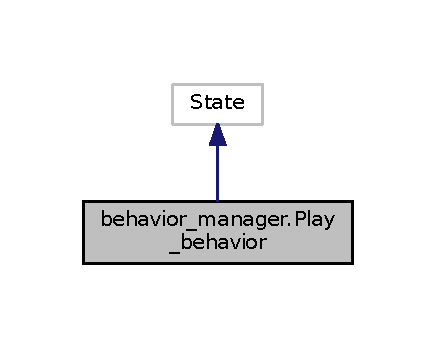
\includegraphics[width=209pt]{classbehavior__manager_1_1Play__behavior__coll__graph}
\end{center}
\end{figure}
\subsection*{Public Member Functions}
\begin{DoxyCompactItemize}
\item 
def \hyperlink{classbehavior__manager_1_1Play__behavior_aaa6ce2b1855d0a235e324df41d8519a1}{\+\_\+\+\_\+init\+\_\+\+\_\+} (self)
\begin{DoxyCompactList}\small\item\em method init \end{DoxyCompactList}\item 
def \hyperlink{classbehavior__manager_1_1Play__behavior_a6c5231ed8f406c82e06c741e89b0f666}{execute} (self, userdata)
\begin{DoxyCompactList}\small\item\em method execute \end{DoxyCompactList}\item 
def \hyperlink{classbehavior__manager_1_1Play__behavior_a575ae46822b1544bd4d0670c2d99782e}{read\+\_\+current\+\_\+location} (self, current\+Room)
\begin{DoxyCompactList}\small\item\em method read\+\_\+current\+\_\+location \end{DoxyCompactList}\end{DoxyCompactItemize}
\subsection*{Public Attributes}
\begin{DoxyCompactItemize}
\item 
\hyperlink{classbehavior__manager_1_1Play__behavior_af636412228a2da30ad114266cbd121e3}{rate}
\item 
\hyperlink{classbehavior__manager_1_1Play__behavior_a8e31d349144e193480484d2a03dd3a7a}{room\+\_\+unknown}
\end{DoxyCompactItemize}


\subsection{Detailed Description}
class \hyperlink{classbehavior__manager_1_1Play__behavior}{Play\+\_\+behavior} 

This class implement the P\+L\+AY behavior of the robot pet It moves the robot to the predefined (X, Y) location within the map and moves it back to the user. The Robot should\+:
\begin{DoxyItemize}
\item start following the ball
\item when the ball stops (it means when the robot stops) it moves the head on the left of 45 degrees, and keep it there for some seconds
\item then it moves the head to the right, stays there for some seconds
\item once moved the head keeps tracking the ball 
\end{DoxyItemize}

\subsection{Constructor \& Destructor Documentation}
\index{behavior\+\_\+manager\+::\+Play\+\_\+behavior@{behavior\+\_\+manager\+::\+Play\+\_\+behavior}!\+\_\+\+\_\+init\+\_\+\+\_\+@{\+\_\+\+\_\+init\+\_\+\+\_\+}}
\index{\+\_\+\+\_\+init\+\_\+\+\_\+@{\+\_\+\+\_\+init\+\_\+\+\_\+}!behavior\+\_\+manager\+::\+Play\+\_\+behavior@{behavior\+\_\+manager\+::\+Play\+\_\+behavior}}
\subsubsection[{\texorpdfstring{\+\_\+\+\_\+init\+\_\+\+\_\+(self)}{__init__(self)}}]{\setlength{\rightskip}{0pt plus 5cm}def behavior\+\_\+manager.\+Play\+\_\+behavior.\+\_\+\+\_\+init\+\_\+\+\_\+ (
\begin{DoxyParamCaption}
\item[{}]{self}
\end{DoxyParamCaption}
)}\hypertarget{classbehavior__manager_1_1Play__behavior_aaa6ce2b1855d0a235e324df41d8519a1}{}\label{classbehavior__manager_1_1Play__behavior_aaa6ce2b1855d0a235e324df41d8519a1}


method init 

it initializes the state class 

\subsection{Member Function Documentation}
\index{behavior\+\_\+manager\+::\+Play\+\_\+behavior@{behavior\+\_\+manager\+::\+Play\+\_\+behavior}!execute@{execute}}
\index{execute@{execute}!behavior\+\_\+manager\+::\+Play\+\_\+behavior@{behavior\+\_\+manager\+::\+Play\+\_\+behavior}}
\subsubsection[{\texorpdfstring{execute(self, userdata)}{execute(self, userdata)}}]{\setlength{\rightskip}{0pt plus 5cm}def behavior\+\_\+manager.\+Play\+\_\+behavior.\+execute (
\begin{DoxyParamCaption}
\item[{}]{self, }
\item[{}]{userdata}
\end{DoxyParamCaption}
)}\hypertarget{classbehavior__manager_1_1Play__behavior_a6c5231ed8f406c82e06c741e89b0f666}{}\label{classbehavior__manager_1_1Play__behavior_a6c5231ed8f406c82e06c741e89b0f666}


method execute 

what the robot should do \index{behavior\+\_\+manager\+::\+Play\+\_\+behavior@{behavior\+\_\+manager\+::\+Play\+\_\+behavior}!read\+\_\+current\+\_\+location@{read\+\_\+current\+\_\+location}}
\index{read\+\_\+current\+\_\+location@{read\+\_\+current\+\_\+location}!behavior\+\_\+manager\+::\+Play\+\_\+behavior@{behavior\+\_\+manager\+::\+Play\+\_\+behavior}}
\subsubsection[{\texorpdfstring{read\+\_\+current\+\_\+location(self, current\+Room)}{read_current_location(self, currentRoom)}}]{\setlength{\rightskip}{0pt plus 5cm}def behavior\+\_\+manager.\+Play\+\_\+behavior.\+read\+\_\+current\+\_\+location (
\begin{DoxyParamCaption}
\item[{}]{self, }
\item[{}]{current\+Room}
\end{DoxyParamCaption}
)}\hypertarget{classbehavior__manager_1_1Play__behavior_a575ae46822b1544bd4d0670c2d99782e}{}\label{classbehavior__manager_1_1Play__behavior_a575ae46822b1544bd4d0670c2d99782e}


method read\+\_\+current\+\_\+location 

subscriber callback to find the ball 

\subsection{Member Data Documentation}
\index{behavior\+\_\+manager\+::\+Play\+\_\+behavior@{behavior\+\_\+manager\+::\+Play\+\_\+behavior}!rate@{rate}}
\index{rate@{rate}!behavior\+\_\+manager\+::\+Play\+\_\+behavior@{behavior\+\_\+manager\+::\+Play\+\_\+behavior}}
\subsubsection[{\texorpdfstring{rate}{rate}}]{\setlength{\rightskip}{0pt plus 5cm}behavior\+\_\+manager.\+Play\+\_\+behavior.\+rate}\hypertarget{classbehavior__manager_1_1Play__behavior_af636412228a2da30ad114266cbd121e3}{}\label{classbehavior__manager_1_1Play__behavior_af636412228a2da30ad114266cbd121e3}
\index{behavior\+\_\+manager\+::\+Play\+\_\+behavior@{behavior\+\_\+manager\+::\+Play\+\_\+behavior}!room\+\_\+unknown@{room\+\_\+unknown}}
\index{room\+\_\+unknown@{room\+\_\+unknown}!behavior\+\_\+manager\+::\+Play\+\_\+behavior@{behavior\+\_\+manager\+::\+Play\+\_\+behavior}}
\subsubsection[{\texorpdfstring{room\+\_\+unknown}{room_unknown}}]{\setlength{\rightskip}{0pt plus 5cm}behavior\+\_\+manager.\+Play\+\_\+behavior.\+room\+\_\+unknown}\hypertarget{classbehavior__manager_1_1Play__behavior_a8e31d349144e193480484d2a03dd3a7a}{}\label{classbehavior__manager_1_1Play__behavior_a8e31d349144e193480484d2a03dd3a7a}


The documentation for this class was generated from the following file\+:\begin{DoxyCompactItemize}
\item 
/home/\+Experimental\+Robotics\+Lab\+Serena/src/exp\+\_\+assignment3/src/\hyperlink{behavior__manager_8py}{behavior\+\_\+manager.\+py}\end{DoxyCompactItemize}

\hypertarget{classbehavior__manager_1_1Sleep__behavior}{}\section{behavior\+\_\+manager.\+Sleep\+\_\+behavior Class Reference}
\label{classbehavior__manager_1_1Sleep__behavior}\index{behavior\+\_\+manager.\+Sleep\+\_\+behavior@{behavior\+\_\+manager.\+Sleep\+\_\+behavior}}


class \hyperlink{classbehavior__manager_1_1Sleep__behavior}{Sleep\+\_\+behavior}  




Inheritance diagram for behavior\+\_\+manager.\+Sleep\+\_\+behavior\+:
\nopagebreak
\begin{figure}[H]
\begin{center}
\leavevmode
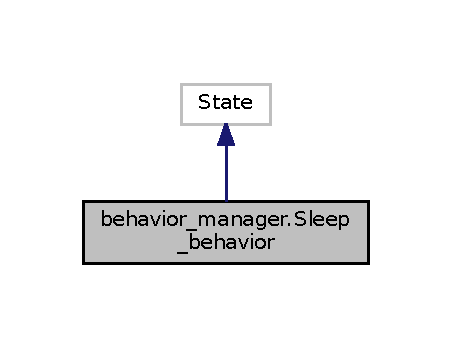
\includegraphics[width=217pt]{classbehavior__manager_1_1Sleep__behavior__inherit__graph}
\end{center}
\end{figure}


Collaboration diagram for behavior\+\_\+manager.\+Sleep\+\_\+behavior\+:
\nopagebreak
\begin{figure}[H]
\begin{center}
\leavevmode
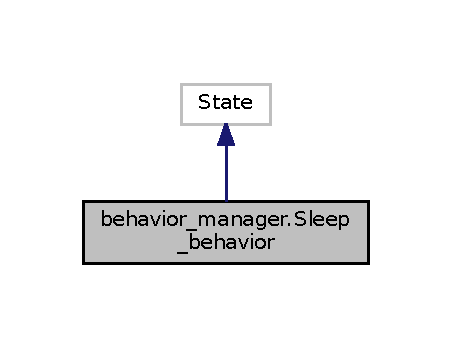
\includegraphics[width=217pt]{classbehavior__manager_1_1Sleep__behavior__coll__graph}
\end{center}
\end{figure}
\subsection*{Public Member Functions}
\begin{DoxyCompactItemize}
\item 
def \hyperlink{classbehavior__manager_1_1Sleep__behavior_a778df3c5a36999ef4792e6ac444bd7f3}{\+\_\+\+\_\+init\+\_\+\+\_\+} (self)
\begin{DoxyCompactList}\small\item\em method init \end{DoxyCompactList}\item 
def \hyperlink{classbehavior__manager_1_1Sleep__behavior_a02d87859cb76d2dbdf78d9d6e2452782}{execute} (self, userdata)
\begin{DoxyCompactList}\small\item\em method execute \end{DoxyCompactList}\item 
def \hyperlink{classbehavior__manager_1_1Sleep__behavior_a06e3c381a9966e030eb82461405d75cf}{check\+\_\+if\+\_\+home\+\_\+position} (self, home)
\begin{DoxyCompactList}\small\item\em method read\+\_\+actual\+\_\+position \end{DoxyCompactList}\end{DoxyCompactItemize}
\subsection*{Public Attributes}
\begin{DoxyCompactItemize}
\item 
\hyperlink{classbehavior__manager_1_1Sleep__behavior_a75cca73975838d3ee66cc687726685de}{rate}
\item 
\hyperlink{classbehavior__manager_1_1Sleep__behavior_ac8a99e565ddf742e5d3d25121bcc99bc}{at\+\_\+home}
\end{DoxyCompactItemize}


\subsection{Detailed Description}
class \hyperlink{classbehavior__manager_1_1Sleep__behavior}{Sleep\+\_\+behavior} 

This class implement the S\+L\+E\+EP behaviour of the robot pet The robot sleeps (S\+L\+E\+EP state)for a random period of time, then it moves to N\+O\+R\+M\+AL state The robot should\+:
\begin{DoxyItemize}
\item reach a predefined location within the arena in Gazebo
\item stays there for some times
\item go back in N\+O\+R\+M\+AL state 
\end{DoxyItemize}

\subsection{Constructor \& Destructor Documentation}
\index{behavior\+\_\+manager\+::\+Sleep\+\_\+behavior@{behavior\+\_\+manager\+::\+Sleep\+\_\+behavior}!\+\_\+\+\_\+init\+\_\+\+\_\+@{\+\_\+\+\_\+init\+\_\+\+\_\+}}
\index{\+\_\+\+\_\+init\+\_\+\+\_\+@{\+\_\+\+\_\+init\+\_\+\+\_\+}!behavior\+\_\+manager\+::\+Sleep\+\_\+behavior@{behavior\+\_\+manager\+::\+Sleep\+\_\+behavior}}
\subsubsection[{\texorpdfstring{\+\_\+\+\_\+init\+\_\+\+\_\+(self)}{__init__(self)}}]{\setlength{\rightskip}{0pt plus 5cm}def behavior\+\_\+manager.\+Sleep\+\_\+behavior.\+\_\+\+\_\+init\+\_\+\+\_\+ (
\begin{DoxyParamCaption}
\item[{}]{self}
\end{DoxyParamCaption}
)}\hypertarget{classbehavior__manager_1_1Sleep__behavior_a778df3c5a36999ef4792e6ac444bd7f3}{}\label{classbehavior__manager_1_1Sleep__behavior_a778df3c5a36999ef4792e6ac444bd7f3}


method init 

it initializes the state class 

\subsection{Member Function Documentation}
\index{behavior\+\_\+manager\+::\+Sleep\+\_\+behavior@{behavior\+\_\+manager\+::\+Sleep\+\_\+behavior}!check\+\_\+if\+\_\+home\+\_\+position@{check\+\_\+if\+\_\+home\+\_\+position}}
\index{check\+\_\+if\+\_\+home\+\_\+position@{check\+\_\+if\+\_\+home\+\_\+position}!behavior\+\_\+manager\+::\+Sleep\+\_\+behavior@{behavior\+\_\+manager\+::\+Sleep\+\_\+behavior}}
\subsubsection[{\texorpdfstring{check\+\_\+if\+\_\+home\+\_\+position(self, home)}{check_if_home_position(self, home)}}]{\setlength{\rightskip}{0pt plus 5cm}def behavior\+\_\+manager.\+Sleep\+\_\+behavior.\+check\+\_\+if\+\_\+home\+\_\+position (
\begin{DoxyParamCaption}
\item[{}]{self, }
\item[{}]{home}
\end{DoxyParamCaption}
)}\hypertarget{classbehavior__manager_1_1Sleep__behavior_a06e3c381a9966e030eb82461405d75cf}{}\label{classbehavior__manager_1_1Sleep__behavior_a06e3c381a9966e030eb82461405d75cf}


method read\+\_\+actual\+\_\+position 

subscriber to actual\+\_\+position\+\_\+robot topic callback, it reads the actual position of the robot \index{behavior\+\_\+manager\+::\+Sleep\+\_\+behavior@{behavior\+\_\+manager\+::\+Sleep\+\_\+behavior}!execute@{execute}}
\index{execute@{execute}!behavior\+\_\+manager\+::\+Sleep\+\_\+behavior@{behavior\+\_\+manager\+::\+Sleep\+\_\+behavior}}
\subsubsection[{\texorpdfstring{execute(self, userdata)}{execute(self, userdata)}}]{\setlength{\rightskip}{0pt plus 5cm}def behavior\+\_\+manager.\+Sleep\+\_\+behavior.\+execute (
\begin{DoxyParamCaption}
\item[{}]{self, }
\item[{}]{userdata}
\end{DoxyParamCaption}
)}\hypertarget{classbehavior__manager_1_1Sleep__behavior_a02d87859cb76d2dbdf78d9d6e2452782}{}\label{classbehavior__manager_1_1Sleep__behavior_a02d87859cb76d2dbdf78d9d6e2452782}


method execute 

This method should
\begin{DoxyItemize}
\item publish \char`\"{}sleep\char`\"{} (String) on the topic behavior
\item check if the robot is already at home position or not 
\end{DoxyItemize}

\subsection{Member Data Documentation}
\index{behavior\+\_\+manager\+::\+Sleep\+\_\+behavior@{behavior\+\_\+manager\+::\+Sleep\+\_\+behavior}!at\+\_\+home@{at\+\_\+home}}
\index{at\+\_\+home@{at\+\_\+home}!behavior\+\_\+manager\+::\+Sleep\+\_\+behavior@{behavior\+\_\+manager\+::\+Sleep\+\_\+behavior}}
\subsubsection[{\texorpdfstring{at\+\_\+home}{at_home}}]{\setlength{\rightskip}{0pt plus 5cm}behavior\+\_\+manager.\+Sleep\+\_\+behavior.\+at\+\_\+home}\hypertarget{classbehavior__manager_1_1Sleep__behavior_ac8a99e565ddf742e5d3d25121bcc99bc}{}\label{classbehavior__manager_1_1Sleep__behavior_ac8a99e565ddf742e5d3d25121bcc99bc}
\index{behavior\+\_\+manager\+::\+Sleep\+\_\+behavior@{behavior\+\_\+manager\+::\+Sleep\+\_\+behavior}!rate@{rate}}
\index{rate@{rate}!behavior\+\_\+manager\+::\+Sleep\+\_\+behavior@{behavior\+\_\+manager\+::\+Sleep\+\_\+behavior}}
\subsubsection[{\texorpdfstring{rate}{rate}}]{\setlength{\rightskip}{0pt plus 5cm}behavior\+\_\+manager.\+Sleep\+\_\+behavior.\+rate}\hypertarget{classbehavior__manager_1_1Sleep__behavior_a75cca73975838d3ee66cc687726685de}{}\label{classbehavior__manager_1_1Sleep__behavior_a75cca73975838d3ee66cc687726685de}


The documentation for this class was generated from the following file\+:\begin{DoxyCompactItemize}
\item 
/home/\+Experimental\+Robotics\+Lab\+Serena/src/exp\+\_\+assignment3/src/\hyperlink{behavior__manager_8py}{behavior\+\_\+manager.\+py}\end{DoxyCompactItemize}

\hypertarget{classopencv__tracking_1_1track__ball}{}\section{opencv\+\_\+tracking.\+track\+\_\+ball Class Reference}
\label{classopencv__tracking_1_1track__ball}\index{opencv\+\_\+tracking.\+track\+\_\+ball@{opencv\+\_\+tracking.\+track\+\_\+ball}}


class \hyperlink{classopencv__tracking_1_1track__ball}{track\+\_\+ball}  


\subsection*{Public Member Functions}
\begin{DoxyCompactItemize}
\item 
def \hyperlink{classopencv__tracking_1_1track__ball_aab7d9901f59d6877955a8d9fbeb1dc0e}{\+\_\+\+\_\+init\+\_\+\+\_\+} (self)
\begin{DoxyCompactList}\small\item\em method {\bfseries init} \end{DoxyCompactList}\item 
def \hyperlink{classopencv__tracking_1_1track__ball_a3f89b28f29c4855aaf8bef0df281c2ef}{get\+\_\+behavior} (self, state)
\begin{DoxyCompactList}\small\item\em method get\+\_\+behavior \end{DoxyCompactList}\item 
def \hyperlink{classopencv__tracking_1_1track__ball_abfde0413e3ed7c7b1c79800e5df78f31}{get\+\_\+room\+\_\+data} (self, \hyperlink{classopencv__tracking_1_1track__ball_a6da54ed7cc2308ea868656753da993ed}{current\+Room})
\begin{DoxyCompactList}\small\item\em method get\+\_\+room\+\_\+data \end{DoxyCompactList}\item 
def \hyperlink{classopencv__tracking_1_1track__ball_ab4cb97ae895654b7e858c102945a20fd}{get\+\_\+odom\+\_\+data} (self, msg)
\begin{DoxyCompactList}\small\item\em method get\+\_\+odom\+\_\+data \end{DoxyCompactList}\item 
def \hyperlink{classopencv__tracking_1_1track__ball_af6054bbfa97909eb6e2ddc115954b6a0}{get\+\_\+laser\+\_\+data} (self, laser)
\begin{DoxyCompactList}\small\item\em method get\+\_\+laser\+\_\+data \end{DoxyCompactList}\item 
def \hyperlink{classopencv__tracking_1_1track__ball_a6a844f8b5d121f37938d9e5c4d1ad44c}{follow\+\_\+ball\+\_\+obstacles} (self)
\begin{DoxyCompactList}\small\item\em method follow\+\_\+ball\+\_\+obstacles \end{DoxyCompactList}\item 
def \hyperlink{classopencv__tracking_1_1track__ball_ac95fc1ff294fdebb621e91067ac3648e}{mask\+\_\+colour\+\_\+function} (self, mask\+Green, mask\+Black, mask\+Red, mask\+Yellow, mask\+Blue, mask\+Magenta)
\begin{DoxyCompactList}\small\item\em method mask\+\_\+colour \end{DoxyCompactList}\item 
def \hyperlink{classopencv__tracking_1_1track__ball_a97b88b8814e8df768a2a80c9e50b73d0}{follow\+\_\+ball} (self)
\begin{DoxyCompactList}\small\item\em method follow\+\_\+ball \end{DoxyCompactList}\item 
def \hyperlink{classopencv__tracking_1_1track__ball_ad0eefbf72841665b36372a1487f54960}{callback} (self, ros\+\_\+data)
\begin{DoxyCompactList}\small\item\em method callback \end{DoxyCompactList}\item 
def \hyperlink{classopencv__tracking_1_1track__ball_ae0d619c1482ceae4077eb958e86cb355}{save\+\_\+position} (self, \hyperlink{classopencv__tracking_1_1track__ball_ad8c66a1a437111152cf8f5797254c0d1}{colour})
\begin{DoxyCompactList}\small\item\em method save\+\_\+position \end{DoxyCompactList}\end{DoxyCompactItemize}
\subsection*{Public Attributes}
\begin{DoxyCompactItemize}
\item 
\hyperlink{classopencv__tracking_1_1track__ball_a2fd263ce72f097474d63022a51a1aff9}{ball\+\_\+visible}
\item 
\hyperlink{classopencv__tracking_1_1track__ball_a38f20351ab0571002f7552aed7bb6979}{near\+\_\+ball}
\item 
\hyperlink{classopencv__tracking_1_1track__ball_a92050fb578b1e2e7bea37b0abdbf26aa}{center}
\begin{DoxyCompactList}\small\item\em cv2 conversion \end{DoxyCompactList}\item 
\hyperlink{classopencv__tracking_1_1track__ball_ae497b649948b1e33fb3cc71b01646da3}{radius}
\item 
\hyperlink{classopencv__tracking_1_1track__ball_ace82efcb5e44b826ac65d61642b447a8}{behaviour}
\item 
\hyperlink{classopencv__tracking_1_1track__ball_aa6598d127ab29a020efbfa871ca23b05}{at\+\_\+ball}
\item 
\hyperlink{classopencv__tracking_1_1track__ball_ad8c66a1a437111152cf8f5797254c0d1}{colour}
\item 
\hyperlink{classopencv__tracking_1_1track__ball_a75f1f4ff39bc26ce8c491ce414f33148}{current\+\_\+position}
\item 
\hyperlink{classopencv__tracking_1_1track__ball_a6da54ed7cc2308ea868656753da993ed}{current\+Room}
\item 
\hyperlink{classopencv__tracking_1_1track__ball_ad2db5078420ea3bf434f25b5dbb961d2}{regions\+\_\+}
\item 
\hyperlink{classopencv__tracking_1_1track__ball_af438ed0f8535d82d07c18b657e19678d}{publisher\+Vel}
\item 
\hyperlink{classopencv__tracking_1_1track__ball_ad351c91525368a89ff0a7bb1d257b3d1}{publisher\+Ball}
\item 
\hyperlink{classopencv__tracking_1_1track__ball_ac5b8f531d5d47698064aafcb9b0a2892}{publisher\+Ball\+Reached}
\item 
\hyperlink{classopencv__tracking_1_1track__ball_a6be8c256872f52e19a7fb0ca60dc61a9}{publisher\+Room}
\item 
\hyperlink{classopencv__tracking_1_1track__ball_a6a59156565d2de7078b22a42f78bea15}{sub\+Cam}
\item 
\hyperlink{classopencv__tracking_1_1track__ball_a4919ca741e094d9679e31c44c58a5295}{sub\+Odom}
\item 
\hyperlink{classopencv__tracking_1_1track__ball_a507d8922c32816d11bc19fadde9ab86c}{sub\+Laser}
\item 
\hyperlink{classopencv__tracking_1_1track__ball_af74c14d19610c2dccedfe19b76680fa6}{sub\+Room}
\item 
\hyperlink{classopencv__tracking_1_1track__ball_aab7a7dae7030c9b39e7bfc1d892b5720}{behavior}
\item 
\hyperlink{classopencv__tracking_1_1track__ball_a82e62d81a3000f65b7aa0d63cd39f129}{regions}
\end{DoxyCompactItemize}


\subsection{Detailed Description}
class \hyperlink{classopencv__tracking_1_1track__ball}{track\+\_\+ball} 

used to track the ball moving in the environment it makes use of cv2 

\subsection{Constructor \& Destructor Documentation}
\index{opencv\+\_\+tracking\+::track\+\_\+ball@{opencv\+\_\+tracking\+::track\+\_\+ball}!\+\_\+\+\_\+init\+\_\+\+\_\+@{\+\_\+\+\_\+init\+\_\+\+\_\+}}
\index{\+\_\+\+\_\+init\+\_\+\+\_\+@{\+\_\+\+\_\+init\+\_\+\+\_\+}!opencv\+\_\+tracking\+::track\+\_\+ball@{opencv\+\_\+tracking\+::track\+\_\+ball}}
\subsubsection[{\texorpdfstring{\+\_\+\+\_\+init\+\_\+\+\_\+(self)}{__init__(self)}}]{\setlength{\rightskip}{0pt plus 5cm}def opencv\+\_\+tracking.\+track\+\_\+ball.\+\_\+\+\_\+init\+\_\+\+\_\+ (
\begin{DoxyParamCaption}
\item[{}]{self}
\end{DoxyParamCaption}
)}\hypertarget{classopencv__tracking_1_1track__ball_aab7d9901f59d6877955a8d9fbeb1dc0e}{}\label{classopencv__tracking_1_1track__ball_aab7d9901f59d6877955a8d9fbeb1dc0e}


method {\bfseries init} 

initialization of the class 

\subsection{Member Function Documentation}
\index{opencv\+\_\+tracking\+::track\+\_\+ball@{opencv\+\_\+tracking\+::track\+\_\+ball}!callback@{callback}}
\index{callback@{callback}!opencv\+\_\+tracking\+::track\+\_\+ball@{opencv\+\_\+tracking\+::track\+\_\+ball}}
\subsubsection[{\texorpdfstring{callback(self, ros\+\_\+data)}{callback(self, ros_data)}}]{\setlength{\rightskip}{0pt plus 5cm}def opencv\+\_\+tracking.\+track\+\_\+ball.\+callback (
\begin{DoxyParamCaption}
\item[{}]{self, }
\item[{}]{ros\+\_\+data}
\end{DoxyParamCaption}
)}\hypertarget{classopencv__tracking_1_1track__ball_ad0eefbf72841665b36372a1487f54960}{}\label{classopencv__tracking_1_1track__ball_ad0eefbf72841665b36372a1487f54960}


method callback 

callback function of topic subscribed we use it to read information on the detection and the converted image \index{opencv\+\_\+tracking\+::track\+\_\+ball@{opencv\+\_\+tracking\+::track\+\_\+ball}!follow\+\_\+ball@{follow\+\_\+ball}}
\index{follow\+\_\+ball@{follow\+\_\+ball}!opencv\+\_\+tracking\+::track\+\_\+ball@{opencv\+\_\+tracking\+::track\+\_\+ball}}
\subsubsection[{\texorpdfstring{follow\+\_\+ball(self)}{follow_ball(self)}}]{\setlength{\rightskip}{0pt plus 5cm}def opencv\+\_\+tracking.\+track\+\_\+ball.\+follow\+\_\+ball (
\begin{DoxyParamCaption}
\item[{}]{self}
\end{DoxyParamCaption}
)}\hypertarget{classopencv__tracking_1_1track__ball_a97b88b8814e8df768a2a80c9e50b73d0}{}\label{classopencv__tracking_1_1track__ball_a97b88b8814e8df768a2a80c9e50b73d0}


method follow\+\_\+ball 

follow the ball \index{opencv\+\_\+tracking\+::track\+\_\+ball@{opencv\+\_\+tracking\+::track\+\_\+ball}!follow\+\_\+ball\+\_\+obstacles@{follow\+\_\+ball\+\_\+obstacles}}
\index{follow\+\_\+ball\+\_\+obstacles@{follow\+\_\+ball\+\_\+obstacles}!opencv\+\_\+tracking\+::track\+\_\+ball@{opencv\+\_\+tracking\+::track\+\_\+ball}}
\subsubsection[{\texorpdfstring{follow\+\_\+ball\+\_\+obstacles(self)}{follow_ball_obstacles(self)}}]{\setlength{\rightskip}{0pt plus 5cm}def opencv\+\_\+tracking.\+track\+\_\+ball.\+follow\+\_\+ball\+\_\+obstacles (
\begin{DoxyParamCaption}
\item[{}]{self}
\end{DoxyParamCaption}
)}\hypertarget{classopencv__tracking_1_1track__ball_a6a844f8b5d121f37938d9e5c4d1ad44c}{}\label{classopencv__tracking_1_1track__ball_a6a844f8b5d121f37938d9e5c4d1ad44c}


method follow\+\_\+ball\+\_\+obstacles 

method to set the robot velocity so that it can follow the ball without hitting obstacles \index{opencv\+\_\+tracking\+::track\+\_\+ball@{opencv\+\_\+tracking\+::track\+\_\+ball}!get\+\_\+behavior@{get\+\_\+behavior}}
\index{get\+\_\+behavior@{get\+\_\+behavior}!opencv\+\_\+tracking\+::track\+\_\+ball@{opencv\+\_\+tracking\+::track\+\_\+ball}}
\subsubsection[{\texorpdfstring{get\+\_\+behavior(self, state)}{get_behavior(self, state)}}]{\setlength{\rightskip}{0pt plus 5cm}def opencv\+\_\+tracking.\+track\+\_\+ball.\+get\+\_\+behavior (
\begin{DoxyParamCaption}
\item[{}]{self, }
\item[{}]{state}
\end{DoxyParamCaption}
)}\hypertarget{classopencv__tracking_1_1track__ball_a3f89b28f29c4855aaf8bef0df281c2ef}{}\label{classopencv__tracking_1_1track__ball_a3f89b28f29c4855aaf8bef0df281c2ef}


method get\+\_\+behavior 

subscriber callback to the behavior topi \index{opencv\+\_\+tracking\+::track\+\_\+ball@{opencv\+\_\+tracking\+::track\+\_\+ball}!get\+\_\+laser\+\_\+data@{get\+\_\+laser\+\_\+data}}
\index{get\+\_\+laser\+\_\+data@{get\+\_\+laser\+\_\+data}!opencv\+\_\+tracking\+::track\+\_\+ball@{opencv\+\_\+tracking\+::track\+\_\+ball}}
\subsubsection[{\texorpdfstring{get\+\_\+laser\+\_\+data(self, laser)}{get_laser_data(self, laser)}}]{\setlength{\rightskip}{0pt plus 5cm}def opencv\+\_\+tracking.\+track\+\_\+ball.\+get\+\_\+laser\+\_\+data (
\begin{DoxyParamCaption}
\item[{}]{self, }
\item[{}]{laser}
\end{DoxyParamCaption}
)}\hypertarget{classopencv__tracking_1_1track__ball_af6054bbfa97909eb6e2ddc115954b6a0}{}\label{classopencv__tracking_1_1track__ball_af6054bbfa97909eb6e2ddc115954b6a0}


method get\+\_\+laser\+\_\+data 

subscriber callback to get laser data \index{opencv\+\_\+tracking\+::track\+\_\+ball@{opencv\+\_\+tracking\+::track\+\_\+ball}!get\+\_\+odom\+\_\+data@{get\+\_\+odom\+\_\+data}}
\index{get\+\_\+odom\+\_\+data@{get\+\_\+odom\+\_\+data}!opencv\+\_\+tracking\+::track\+\_\+ball@{opencv\+\_\+tracking\+::track\+\_\+ball}}
\subsubsection[{\texorpdfstring{get\+\_\+odom\+\_\+data(self, msg)}{get_odom_data(self, msg)}}]{\setlength{\rightskip}{0pt plus 5cm}def opencv\+\_\+tracking.\+track\+\_\+ball.\+get\+\_\+odom\+\_\+data (
\begin{DoxyParamCaption}
\item[{}]{self, }
\item[{}]{msg}
\end{DoxyParamCaption}
)}\hypertarget{classopencv__tracking_1_1track__ball_ab4cb97ae895654b7e858c102945a20fd}{}\label{classopencv__tracking_1_1track__ball_ab4cb97ae895654b7e858c102945a20fd}


method get\+\_\+odom\+\_\+data 

subscriber callback to get odometry of the robot \index{opencv\+\_\+tracking\+::track\+\_\+ball@{opencv\+\_\+tracking\+::track\+\_\+ball}!get\+\_\+room\+\_\+data@{get\+\_\+room\+\_\+data}}
\index{get\+\_\+room\+\_\+data@{get\+\_\+room\+\_\+data}!opencv\+\_\+tracking\+::track\+\_\+ball@{opencv\+\_\+tracking\+::track\+\_\+ball}}
\subsubsection[{\texorpdfstring{get\+\_\+room\+\_\+data(self, current\+Room)}{get_room_data(self, currentRoom)}}]{\setlength{\rightskip}{0pt plus 5cm}def opencv\+\_\+tracking.\+track\+\_\+ball.\+get\+\_\+room\+\_\+data (
\begin{DoxyParamCaption}
\item[{}]{self, }
\item[{}]{current\+Room}
\end{DoxyParamCaption}
)}\hypertarget{classopencv__tracking_1_1track__ball_abfde0413e3ed7c7b1c79800e5df78f31}{}\label{classopencv__tracking_1_1track__ball_abfde0413e3ed7c7b1c79800e5df78f31}


method get\+\_\+room\+\_\+data 

subscriber callback to get current room \index{opencv\+\_\+tracking\+::track\+\_\+ball@{opencv\+\_\+tracking\+::track\+\_\+ball}!mask\+\_\+colour\+\_\+function@{mask\+\_\+colour\+\_\+function}}
\index{mask\+\_\+colour\+\_\+function@{mask\+\_\+colour\+\_\+function}!opencv\+\_\+tracking\+::track\+\_\+ball@{opencv\+\_\+tracking\+::track\+\_\+ball}}
\subsubsection[{\texorpdfstring{mask\+\_\+colour\+\_\+function(self, mask\+Green, mask\+Black, mask\+Red, mask\+Yellow, mask\+Blue, mask\+Magenta)}{mask_colour_function(self, maskGreen, maskBlack, maskRed, maskYellow, maskBlue, maskMagenta)}}]{\setlength{\rightskip}{0pt plus 5cm}def opencv\+\_\+tracking.\+track\+\_\+ball.\+mask\+\_\+colour\+\_\+function (
\begin{DoxyParamCaption}
\item[{}]{self, }
\item[{}]{mask\+Green, }
\item[{}]{mask\+Black, }
\item[{}]{mask\+Red, }
\item[{}]{mask\+Yellow, }
\item[{}]{mask\+Blue, }
\item[{}]{mask\+Magenta}
\end{DoxyParamCaption}
)}\hypertarget{classopencv__tracking_1_1track__ball_ac95fc1ff294fdebb621e91067ac3648e}{}\label{classopencv__tracking_1_1track__ball_ac95fc1ff294fdebb621e91067ac3648e}


method mask\+\_\+colour 

method to decide which colour \index{opencv\+\_\+tracking\+::track\+\_\+ball@{opencv\+\_\+tracking\+::track\+\_\+ball}!save\+\_\+position@{save\+\_\+position}}
\index{save\+\_\+position@{save\+\_\+position}!opencv\+\_\+tracking\+::track\+\_\+ball@{opencv\+\_\+tracking\+::track\+\_\+ball}}
\subsubsection[{\texorpdfstring{save\+\_\+position(self, colour)}{save_position(self, colour)}}]{\setlength{\rightskip}{0pt plus 5cm}def opencv\+\_\+tracking.\+track\+\_\+ball.\+save\+\_\+position (
\begin{DoxyParamCaption}
\item[{}]{self, }
\item[{}]{colour}
\end{DoxyParamCaption}
)}\hypertarget{classopencv__tracking_1_1track__ball_ae0d619c1482ceae4077eb958e86cb355}{}\label{classopencv__tracking_1_1track__ball_ae0d619c1482ceae4077eb958e86cb355}


method save\+\_\+position 

Saves the position of the tracked ball 

\subsection{Member Data Documentation}
\index{opencv\+\_\+tracking\+::track\+\_\+ball@{opencv\+\_\+tracking\+::track\+\_\+ball}!at\+\_\+ball@{at\+\_\+ball}}
\index{at\+\_\+ball@{at\+\_\+ball}!opencv\+\_\+tracking\+::track\+\_\+ball@{opencv\+\_\+tracking\+::track\+\_\+ball}}
\subsubsection[{\texorpdfstring{at\+\_\+ball}{at_ball}}]{\setlength{\rightskip}{0pt plus 5cm}opencv\+\_\+tracking.\+track\+\_\+ball.\+at\+\_\+ball}\hypertarget{classopencv__tracking_1_1track__ball_aa6598d127ab29a020efbfa871ca23b05}{}\label{classopencv__tracking_1_1track__ball_aa6598d127ab29a020efbfa871ca23b05}
\index{opencv\+\_\+tracking\+::track\+\_\+ball@{opencv\+\_\+tracking\+::track\+\_\+ball}!ball\+\_\+visible@{ball\+\_\+visible}}
\index{ball\+\_\+visible@{ball\+\_\+visible}!opencv\+\_\+tracking\+::track\+\_\+ball@{opencv\+\_\+tracking\+::track\+\_\+ball}}
\subsubsection[{\texorpdfstring{ball\+\_\+visible}{ball_visible}}]{\setlength{\rightskip}{0pt plus 5cm}opencv\+\_\+tracking.\+track\+\_\+ball.\+ball\+\_\+visible}\hypertarget{classopencv__tracking_1_1track__ball_a2fd263ce72f097474d63022a51a1aff9}{}\label{classopencv__tracking_1_1track__ball_a2fd263ce72f097474d63022a51a1aff9}
\index{opencv\+\_\+tracking\+::track\+\_\+ball@{opencv\+\_\+tracking\+::track\+\_\+ball}!behavior@{behavior}}
\index{behavior@{behavior}!opencv\+\_\+tracking\+::track\+\_\+ball@{opencv\+\_\+tracking\+::track\+\_\+ball}}
\subsubsection[{\texorpdfstring{behavior}{behavior}}]{\setlength{\rightskip}{0pt plus 5cm}opencv\+\_\+tracking.\+track\+\_\+ball.\+behavior}\hypertarget{classopencv__tracking_1_1track__ball_aab7a7dae7030c9b39e7bfc1d892b5720}{}\label{classopencv__tracking_1_1track__ball_aab7a7dae7030c9b39e7bfc1d892b5720}
\index{opencv\+\_\+tracking\+::track\+\_\+ball@{opencv\+\_\+tracking\+::track\+\_\+ball}!behaviour@{behaviour}}
\index{behaviour@{behaviour}!opencv\+\_\+tracking\+::track\+\_\+ball@{opencv\+\_\+tracking\+::track\+\_\+ball}}
\subsubsection[{\texorpdfstring{behaviour}{behaviour}}]{\setlength{\rightskip}{0pt plus 5cm}opencv\+\_\+tracking.\+track\+\_\+ball.\+behaviour}\hypertarget{classopencv__tracking_1_1track__ball_ace82efcb5e44b826ac65d61642b447a8}{}\label{classopencv__tracking_1_1track__ball_ace82efcb5e44b826ac65d61642b447a8}
\index{opencv\+\_\+tracking\+::track\+\_\+ball@{opencv\+\_\+tracking\+::track\+\_\+ball}!center@{center}}
\index{center@{center}!opencv\+\_\+tracking\+::track\+\_\+ball@{opencv\+\_\+tracking\+::track\+\_\+ball}}
\subsubsection[{\texorpdfstring{center}{center}}]{\setlength{\rightskip}{0pt plus 5cm}opencv\+\_\+tracking.\+track\+\_\+ball.\+center}\hypertarget{classopencv__tracking_1_1track__ball_a92050fb578b1e2e7bea37b0abdbf26aa}{}\label{classopencv__tracking_1_1track__ball_a92050fb578b1e2e7bea37b0abdbf26aa}


cv2 conversion 

\index{opencv\+\_\+tracking\+::track\+\_\+ball@{opencv\+\_\+tracking\+::track\+\_\+ball}!colour@{colour}}
\index{colour@{colour}!opencv\+\_\+tracking\+::track\+\_\+ball@{opencv\+\_\+tracking\+::track\+\_\+ball}}
\subsubsection[{\texorpdfstring{colour}{colour}}]{\setlength{\rightskip}{0pt plus 5cm}opencv\+\_\+tracking.\+track\+\_\+ball.\+colour}\hypertarget{classopencv__tracking_1_1track__ball_ad8c66a1a437111152cf8f5797254c0d1}{}\label{classopencv__tracking_1_1track__ball_ad8c66a1a437111152cf8f5797254c0d1}
\index{opencv\+\_\+tracking\+::track\+\_\+ball@{opencv\+\_\+tracking\+::track\+\_\+ball}!current\+\_\+position@{current\+\_\+position}}
\index{current\+\_\+position@{current\+\_\+position}!opencv\+\_\+tracking\+::track\+\_\+ball@{opencv\+\_\+tracking\+::track\+\_\+ball}}
\subsubsection[{\texorpdfstring{current\+\_\+position}{current_position}}]{\setlength{\rightskip}{0pt plus 5cm}opencv\+\_\+tracking.\+track\+\_\+ball.\+current\+\_\+position}\hypertarget{classopencv__tracking_1_1track__ball_a75f1f4ff39bc26ce8c491ce414f33148}{}\label{classopencv__tracking_1_1track__ball_a75f1f4ff39bc26ce8c491ce414f33148}
\index{opencv\+\_\+tracking\+::track\+\_\+ball@{opencv\+\_\+tracking\+::track\+\_\+ball}!current\+Room@{current\+Room}}
\index{current\+Room@{current\+Room}!opencv\+\_\+tracking\+::track\+\_\+ball@{opencv\+\_\+tracking\+::track\+\_\+ball}}
\subsubsection[{\texorpdfstring{current\+Room}{currentRoom}}]{\setlength{\rightskip}{0pt plus 5cm}opencv\+\_\+tracking.\+track\+\_\+ball.\+current\+Room}\hypertarget{classopencv__tracking_1_1track__ball_a6da54ed7cc2308ea868656753da993ed}{}\label{classopencv__tracking_1_1track__ball_a6da54ed7cc2308ea868656753da993ed}
\index{opencv\+\_\+tracking\+::track\+\_\+ball@{opencv\+\_\+tracking\+::track\+\_\+ball}!near\+\_\+ball@{near\+\_\+ball}}
\index{near\+\_\+ball@{near\+\_\+ball}!opencv\+\_\+tracking\+::track\+\_\+ball@{opencv\+\_\+tracking\+::track\+\_\+ball}}
\subsubsection[{\texorpdfstring{near\+\_\+ball}{near_ball}}]{\setlength{\rightskip}{0pt plus 5cm}opencv\+\_\+tracking.\+track\+\_\+ball.\+near\+\_\+ball}\hypertarget{classopencv__tracking_1_1track__ball_a38f20351ab0571002f7552aed7bb6979}{}\label{classopencv__tracking_1_1track__ball_a38f20351ab0571002f7552aed7bb6979}
\index{opencv\+\_\+tracking\+::track\+\_\+ball@{opencv\+\_\+tracking\+::track\+\_\+ball}!publisher\+Ball@{publisher\+Ball}}
\index{publisher\+Ball@{publisher\+Ball}!opencv\+\_\+tracking\+::track\+\_\+ball@{opencv\+\_\+tracking\+::track\+\_\+ball}}
\subsubsection[{\texorpdfstring{publisher\+Ball}{publisherBall}}]{\setlength{\rightskip}{0pt plus 5cm}opencv\+\_\+tracking.\+track\+\_\+ball.\+publisher\+Ball}\hypertarget{classopencv__tracking_1_1track__ball_ad351c91525368a89ff0a7bb1d257b3d1}{}\label{classopencv__tracking_1_1track__ball_ad351c91525368a89ff0a7bb1d257b3d1}
\index{opencv\+\_\+tracking\+::track\+\_\+ball@{opencv\+\_\+tracking\+::track\+\_\+ball}!publisher\+Ball\+Reached@{publisher\+Ball\+Reached}}
\index{publisher\+Ball\+Reached@{publisher\+Ball\+Reached}!opencv\+\_\+tracking\+::track\+\_\+ball@{opencv\+\_\+tracking\+::track\+\_\+ball}}
\subsubsection[{\texorpdfstring{publisher\+Ball\+Reached}{publisherBallReached}}]{\setlength{\rightskip}{0pt plus 5cm}opencv\+\_\+tracking.\+track\+\_\+ball.\+publisher\+Ball\+Reached}\hypertarget{classopencv__tracking_1_1track__ball_ac5b8f531d5d47698064aafcb9b0a2892}{}\label{classopencv__tracking_1_1track__ball_ac5b8f531d5d47698064aafcb9b0a2892}
\index{opencv\+\_\+tracking\+::track\+\_\+ball@{opencv\+\_\+tracking\+::track\+\_\+ball}!publisher\+Room@{publisher\+Room}}
\index{publisher\+Room@{publisher\+Room}!opencv\+\_\+tracking\+::track\+\_\+ball@{opencv\+\_\+tracking\+::track\+\_\+ball}}
\subsubsection[{\texorpdfstring{publisher\+Room}{publisherRoom}}]{\setlength{\rightskip}{0pt plus 5cm}opencv\+\_\+tracking.\+track\+\_\+ball.\+publisher\+Room}\hypertarget{classopencv__tracking_1_1track__ball_a6be8c256872f52e19a7fb0ca60dc61a9}{}\label{classopencv__tracking_1_1track__ball_a6be8c256872f52e19a7fb0ca60dc61a9}
\index{opencv\+\_\+tracking\+::track\+\_\+ball@{opencv\+\_\+tracking\+::track\+\_\+ball}!publisher\+Vel@{publisher\+Vel}}
\index{publisher\+Vel@{publisher\+Vel}!opencv\+\_\+tracking\+::track\+\_\+ball@{opencv\+\_\+tracking\+::track\+\_\+ball}}
\subsubsection[{\texorpdfstring{publisher\+Vel}{publisherVel}}]{\setlength{\rightskip}{0pt plus 5cm}opencv\+\_\+tracking.\+track\+\_\+ball.\+publisher\+Vel}\hypertarget{classopencv__tracking_1_1track__ball_af438ed0f8535d82d07c18b657e19678d}{}\label{classopencv__tracking_1_1track__ball_af438ed0f8535d82d07c18b657e19678d}
\index{opencv\+\_\+tracking\+::track\+\_\+ball@{opencv\+\_\+tracking\+::track\+\_\+ball}!radius@{radius}}
\index{radius@{radius}!opencv\+\_\+tracking\+::track\+\_\+ball@{opencv\+\_\+tracking\+::track\+\_\+ball}}
\subsubsection[{\texorpdfstring{radius}{radius}}]{\setlength{\rightskip}{0pt plus 5cm}opencv\+\_\+tracking.\+track\+\_\+ball.\+radius}\hypertarget{classopencv__tracking_1_1track__ball_ae497b649948b1e33fb3cc71b01646da3}{}\label{classopencv__tracking_1_1track__ball_ae497b649948b1e33fb3cc71b01646da3}
\index{opencv\+\_\+tracking\+::track\+\_\+ball@{opencv\+\_\+tracking\+::track\+\_\+ball}!regions@{regions}}
\index{regions@{regions}!opencv\+\_\+tracking\+::track\+\_\+ball@{opencv\+\_\+tracking\+::track\+\_\+ball}}
\subsubsection[{\texorpdfstring{regions}{regions}}]{\setlength{\rightskip}{0pt plus 5cm}opencv\+\_\+tracking.\+track\+\_\+ball.\+regions}\hypertarget{classopencv__tracking_1_1track__ball_a82e62d81a3000f65b7aa0d63cd39f129}{}\label{classopencv__tracking_1_1track__ball_a82e62d81a3000f65b7aa0d63cd39f129}
\index{opencv\+\_\+tracking\+::track\+\_\+ball@{opencv\+\_\+tracking\+::track\+\_\+ball}!regions\+\_\+@{regions\+\_\+}}
\index{regions\+\_\+@{regions\+\_\+}!opencv\+\_\+tracking\+::track\+\_\+ball@{opencv\+\_\+tracking\+::track\+\_\+ball}}
\subsubsection[{\texorpdfstring{regions\+\_\+}{regions_}}]{\setlength{\rightskip}{0pt plus 5cm}opencv\+\_\+tracking.\+track\+\_\+ball.\+regions\+\_\+}\hypertarget{classopencv__tracking_1_1track__ball_ad2db5078420ea3bf434f25b5dbb961d2}{}\label{classopencv__tracking_1_1track__ball_ad2db5078420ea3bf434f25b5dbb961d2}
\index{opencv\+\_\+tracking\+::track\+\_\+ball@{opencv\+\_\+tracking\+::track\+\_\+ball}!sub\+Cam@{sub\+Cam}}
\index{sub\+Cam@{sub\+Cam}!opencv\+\_\+tracking\+::track\+\_\+ball@{opencv\+\_\+tracking\+::track\+\_\+ball}}
\subsubsection[{\texorpdfstring{sub\+Cam}{subCam}}]{\setlength{\rightskip}{0pt plus 5cm}opencv\+\_\+tracking.\+track\+\_\+ball.\+sub\+Cam}\hypertarget{classopencv__tracking_1_1track__ball_a6a59156565d2de7078b22a42f78bea15}{}\label{classopencv__tracking_1_1track__ball_a6a59156565d2de7078b22a42f78bea15}
\index{opencv\+\_\+tracking\+::track\+\_\+ball@{opencv\+\_\+tracking\+::track\+\_\+ball}!sub\+Laser@{sub\+Laser}}
\index{sub\+Laser@{sub\+Laser}!opencv\+\_\+tracking\+::track\+\_\+ball@{opencv\+\_\+tracking\+::track\+\_\+ball}}
\subsubsection[{\texorpdfstring{sub\+Laser}{subLaser}}]{\setlength{\rightskip}{0pt plus 5cm}opencv\+\_\+tracking.\+track\+\_\+ball.\+sub\+Laser}\hypertarget{classopencv__tracking_1_1track__ball_a507d8922c32816d11bc19fadde9ab86c}{}\label{classopencv__tracking_1_1track__ball_a507d8922c32816d11bc19fadde9ab86c}
\index{opencv\+\_\+tracking\+::track\+\_\+ball@{opencv\+\_\+tracking\+::track\+\_\+ball}!sub\+Odom@{sub\+Odom}}
\index{sub\+Odom@{sub\+Odom}!opencv\+\_\+tracking\+::track\+\_\+ball@{opencv\+\_\+tracking\+::track\+\_\+ball}}
\subsubsection[{\texorpdfstring{sub\+Odom}{subOdom}}]{\setlength{\rightskip}{0pt plus 5cm}opencv\+\_\+tracking.\+track\+\_\+ball.\+sub\+Odom}\hypertarget{classopencv__tracking_1_1track__ball_a4919ca741e094d9679e31c44c58a5295}{}\label{classopencv__tracking_1_1track__ball_a4919ca741e094d9679e31c44c58a5295}
\index{opencv\+\_\+tracking\+::track\+\_\+ball@{opencv\+\_\+tracking\+::track\+\_\+ball}!sub\+Room@{sub\+Room}}
\index{sub\+Room@{sub\+Room}!opencv\+\_\+tracking\+::track\+\_\+ball@{opencv\+\_\+tracking\+::track\+\_\+ball}}
\subsubsection[{\texorpdfstring{sub\+Room}{subRoom}}]{\setlength{\rightskip}{0pt plus 5cm}opencv\+\_\+tracking.\+track\+\_\+ball.\+sub\+Room}\hypertarget{classopencv__tracking_1_1track__ball_af74c14d19610c2dccedfe19b76680fa6}{}\label{classopencv__tracking_1_1track__ball_af74c14d19610c2dccedfe19b76680fa6}


The documentation for this class was generated from the following file\+:\begin{DoxyCompactItemize}
\item 
/home/\+Experimental\+Robotics\+Lab\+Serena/src/exp\+\_\+assignment3/src/\hyperlink{opencv__tracking_8py}{opencv\+\_\+tracking.\+py}\end{DoxyCompactItemize}

\chapter{File Documentation}
\hypertarget{behavior__manager_8py}{}\section{/home/\+Experimental\+Robotics\+Lab\+Serena/src/exp\+\_\+assignment3/src/behavior\+\_\+manager.py File Reference}
\label{behavior__manager_8py}\index{/home/\+Experimental\+Robotics\+Lab\+Serena/src/exp\+\_\+assignment3/src/behavior\+\_\+manager.\+py@{/home/\+Experimental\+Robotics\+Lab\+Serena/src/exp\+\_\+assignment3/src/behavior\+\_\+manager.\+py}}
\subsection*{Classes}
\begin{DoxyCompactItemize}
\item 
class \hyperlink{classbehavior__manager_1_1Normal__behavior}{behavior\+\_\+manager.\+Normal\+\_\+behavior}
\begin{DoxyCompactList}\small\item\em class \hyperlink{classbehavior__manager_1_1Normal__behavior}{Normal\+\_\+behavior} \end{DoxyCompactList}\item 
class \hyperlink{classbehavior__manager_1_1Normal__track__behaviour}{behavior\+\_\+manager.\+Normal\+\_\+track\+\_\+behaviour}
\begin{DoxyCompactList}\small\item\em class \hyperlink{classbehavior__manager_1_1Normal__track__behaviour}{Normal\+\_\+track\+\_\+behaviour} \end{DoxyCompactList}\item 
class \hyperlink{classbehavior__manager_1_1Find__track__behaviour}{behavior\+\_\+manager.\+Find\+\_\+track\+\_\+behaviour}
\begin{DoxyCompactList}\small\item\em class \hyperlink{classbehavior__manager_1_1Find__track__behaviour}{Find\+\_\+track\+\_\+behaviour} \end{DoxyCompactList}\item 
class \hyperlink{classbehavior__manager_1_1Sleep__behavior}{behavior\+\_\+manager.\+Sleep\+\_\+behavior}
\begin{DoxyCompactList}\small\item\em class \hyperlink{classbehavior__manager_1_1Sleep__behavior}{Sleep\+\_\+behavior} \end{DoxyCompactList}\item 
class \hyperlink{classbehavior__manager_1_1Play__behavior}{behavior\+\_\+manager.\+Play\+\_\+behavior}
\begin{DoxyCompactList}\small\item\em class \hyperlink{classbehavior__manager_1_1Play__behavior}{Play\+\_\+behavior} \end{DoxyCompactList}\item 
class \hyperlink{classbehavior__manager_1_1Find__behavior}{behavior\+\_\+manager.\+Find\+\_\+behavior}
\begin{DoxyCompactList}\small\item\em class \hyperlink{classbehavior__manager_1_1Find__behavior}{Find\+\_\+behavior} \end{DoxyCompactList}\end{DoxyCompactItemize}
\subsection*{Namespaces}
\begin{DoxyCompactItemize}
\item 
 \hyperlink{namespacebehavior__manager}{behavior\+\_\+manager}
\begin{DoxyCompactList}\small\item\em Here is implemented the state machine that controls the switch between the behaviours of the robot. \end{DoxyCompactList}\end{DoxyCompactItemize}
\subsection*{Functions}
\begin{DoxyCompactItemize}
\item 
def \hyperlink{namespacebehavior__manager_a81416c498199e9a8bc275514afaf9944}{behavior\+\_\+manager.\+main} ()
\begin{DoxyCompactList}\small\item\em function main \end{DoxyCompactList}\end{DoxyCompactItemize}
\subsection*{Variables}
\begin{DoxyCompactItemize}
\item 
\hyperlink{namespacebehavior__manager_ac30069bca00035c62a13df72bf29a3aa}{behavior\+\_\+manager.\+pub\+\_\+behavior} = rospy.\+Publisher(\char`\"{}/behavior\char`\"{}, String, queue\+\_\+size=1)
\begin{DoxyCompactList}\small\item\em publisher pub\+\_\+behavior \end{DoxyCompactList}\end{DoxyCompactItemize}

\hypertarget{human__simulator_8py}{}\section{/home/\+Experimental\+Robotics\+Lab\+Serena/src/exp\+\_\+assignment3/src/human\+\_\+simulator.py File Reference}
\label{human__simulator_8py}\index{/home/\+Experimental\+Robotics\+Lab\+Serena/src/exp\+\_\+assignment3/src/human\+\_\+simulator.\+py@{/home/\+Experimental\+Robotics\+Lab\+Serena/src/exp\+\_\+assignment3/src/human\+\_\+simulator.\+py}}
\subsection*{Namespaces}
\begin{DoxyCompactItemize}
\item 
 \hyperlink{namespacehuman__simulator}{human\+\_\+simulator}
\begin{DoxyCompactList}\small\item\em Human interactions with the ball The human can\+: 1) move the ball around. \end{DoxyCompactList}\end{DoxyCompactItemize}
\subsection*{Functions}
\begin{DoxyCompactItemize}
\item 
def \hyperlink{namespacehuman__simulator_aaf8bac689897648e75aeb3f194e6cde1}{human\+\_\+simulator.\+get\+\_\+room\+\_\+position} ()
\begin{DoxyCompactList}\small\item\em function get\+\_\+random\+\_\+position \end{DoxyCompactList}\item 
def \hyperlink{namespacehuman__simulator_a1ffee3228c32e64a7d458b86b00e8a55}{human\+\_\+simulator.\+check\+\_\+at\+\_\+human} (home)
\begin{DoxyCompactList}\small\item\em function \hyperlink{namespacehuman__simulator_a1ffee3228c32e64a7d458b86b00e8a55}{check\+\_\+at\+\_\+human()} \end{DoxyCompactList}\item 
def \hyperlink{namespacehuman__simulator_adb91dbb164188ff85ca65a1c0380a16a}{human\+\_\+simulator.\+main} ()
\begin{DoxyCompactList}\small\item\em main function \end{DoxyCompactList}\end{DoxyCompactItemize}
\subsection*{Variables}
\begin{DoxyCompactItemize}
\item 
\hyperlink{namespacehuman__simulator_a7ab8519bbc715b4fc0be38fca89bb1ea}{human\+\_\+simulator.\+publisher\+Play} = None
\item 
\hyperlink{namespacehuman__simulator_abf72cf6c41334f67acbd3a64400611b9}{human\+\_\+simulator.\+publisher\+Command\+Room} = None
\item 
\hyperlink{namespacehuman__simulator_a1d29f5a2849453421e867b733b0d9f3f}{human\+\_\+simulator.\+at\+\_\+human} = None
\end{DoxyCompactItemize}

\hypertarget{motion_8py}{}\section{/home/\+Experimental\+Robotics\+Lab\+Serena/src/exp\+\_\+assignment3/src/motion.py File Reference}
\label{motion_8py}\index{/home/\+Experimental\+Robotics\+Lab\+Serena/src/exp\+\_\+assignment3/src/motion.\+py@{/home/\+Experimental\+Robotics\+Lab\+Serena/src/exp\+\_\+assignment3/src/motion.\+py}}
\subsection*{Namespaces}
\begin{DoxyCompactItemize}
\item 
 \hyperlink{namespacemotion}{motion}
\begin{DoxyCompactList}\small\item\em It moves the robot within the Gazebo environment according to the given behavior. \end{DoxyCompactList}\end{DoxyCompactItemize}
\subsection*{Functions}
\begin{DoxyCompactItemize}
\item 
def \hyperlink{namespacemotion_af838e21dbf42903e9919b1b9263e306c}{motion.\+get\+\_\+random\+\_\+position} ()
\begin{DoxyCompactList}\small\item\em function random position on map \end{DoxyCompactList}\item 
def \hyperlink{namespacemotion_aa4861fa33d9ce9a5edf2e9c5d0393ec1}{motion.\+get\+\_\+current\+\_\+room\+\_\+position} ()
\begin{DoxyCompactList}\small\item\em function get\+\_\+current\+\_\+room\+\_\+position \end{DoxyCompactList}\item 
def \hyperlink{namespacemotion_a780223b6acd6bda378971227650c92e1}{motion.\+callback\+\_\+get\+\_\+behaviour} (state)
\begin{DoxyCompactList}\small\item\em function callback\+\_\+get\+\_\+behavior \end{DoxyCompactList}\item 
def \hyperlink{namespacemotion_ae3d3508540404a8a6e74b2808768e95d}{motion.\+get\+\_\+room\+\_\+command} (human\+\_\+command)
\begin{DoxyCompactList}\small\item\em function get\+\_\+room\+\_\+command \end{DoxyCompactList}\item 
def \hyperlink{namespacemotion_a4d516c2d2b3bec18bb4c6faf73e38fc8}{motion.\+feedback\+\_\+cb} (check)
\begin{DoxyCompactList}\small\item\em function feedback\+\_\+cb \end{DoxyCompactList}\item 
def \hyperlink{namespacemotion_ad19c84db008ed0163c8122d570d026e2}{motion.\+move\+\_\+random\+\_\+normal} ()
\begin{DoxyCompactList}\small\item\em function move\+\_\+normal \end{DoxyCompactList}\item 
def \hyperlink{namespacemotion_a7e28371ac015cdd23c39095626abce98}{motion.\+move\+\_\+sleep\+\_\+position} ()
\begin{DoxyCompactList}\small\item\em function move\+\_\+sleep\+\_\+position \end{DoxyCompactList}\item 
def \hyperlink{namespacemotion_a8291fff74d22580af44a2c7cb56eaeeb}{motion.\+play\+\_\+motion} ()
\begin{DoxyCompactList}\small\item\em function play\+\_\+motion \end{DoxyCompactList}\item 
def \hyperlink{namespacemotion_ad6289fca8572f5af95fd28f4c2dbc68d}{motion.\+main} ()
\begin{DoxyCompactList}\small\item\em function main \end{DoxyCompactList}\end{DoxyCompactItemize}
\subsection*{Variables}
\begin{DoxyCompactItemize}
\item 
bool \hyperlink{namespacemotion_a9f9cd0f38a0aad33b5304b4edef120cd}{motion.\+V\+E\+R\+B\+O\+SE} = False
\item 
\hyperlink{namespacemotion_a15d63b2a70ac940f179085ce72871c86}{motion.\+behaviour} = None
\begin{DoxyCompactList}\small\item\em global variables initialize behavior \end{DoxyCompactList}\item 
\hyperlink{namespacemotion_ac7315ec450891f4f81a17315dccc7903}{motion.\+current\+Room} = None
\item 
\hyperlink{namespacemotion_a635c1fd35291e93dc73ab2f6c6f7c8c4}{motion.\+current\+Room\+Pos} = None
\item 
list \hyperlink{namespacemotion_aa995e8257b20bb286a59bf6bb3c5f375}{motion.\+home\+\_\+position} = \mbox{[}rospy.\+get\+\_\+param(\textquotesingle{}home\+\_\+x\textquotesingle{}), rospy.\+get\+\_\+param(\textquotesingle{}home\+\_\+y\textquotesingle{})\mbox{]}
\item 
\hyperlink{namespacemotion_aba6af569cf57bbdc8a1d01598d29d99b}{motion.\+act\+\_\+c} = None
\item 
\hyperlink{namespacemotion_aa7760f4160a77a04d3cc60233ad138ab}{motion.\+publisher\+At\+Home} = rospy.\+Publisher(\char`\"{}/at\+\_\+home\char`\"{}, Bool, queue\+\_\+size=1)
\item 
\hyperlink{namespacemotion_a11a206a594fcaf6dff8429664bcce376}{motion.\+publisher\+At\+Human} = rospy.\+Publisher(\char`\"{}/at\+\_\+human\char`\"{}, Bool, queue\+\_\+size=1)
\item 
\hyperlink{namespacemotion_ac08467b50a1ebb7e985d8b93bcf5653d}{motion.\+publisher\+Unknown\+Room} = rospy.\+Publisher(\char`\"{}/unknown\+\_\+room\char`\"{}, Bool, queue\+\_\+size=1)
\item 
bool \hyperlink{namespacemotion_a30e58643e988d1faddb84cdfd54965f8}{motion.\+at\+\_\+home} = False
\item 
bool \hyperlink{namespacemotion_a8a70e4c3b029440acf94460c95f42841}{motion.\+at\+\_\+human} = False
\item 
\hyperlink{namespacemotion_a86619454560e5d6f8dfe5dd042391ca1}{motion.\+rate} = None
\end{DoxyCompactItemize}

\hypertarget{opencv__tracking_8py}{}\section{/home/\+Experimental\+Robotics\+Lab\+Serena/src/exp\+\_\+assignment3/src/opencv\+\_\+tracking.py File Reference}
\label{opencv__tracking_8py}\index{/home/\+Experimental\+Robotics\+Lab\+Serena/src/exp\+\_\+assignment3/src/opencv\+\_\+tracking.\+py@{/home/\+Experimental\+Robotics\+Lab\+Serena/src/exp\+\_\+assignment3/src/opencv\+\_\+tracking.\+py}}
\subsection*{Classes}
\begin{DoxyCompactItemize}
\item 
class \hyperlink{classopencv__tracking_1_1track__ball}{opencv\+\_\+tracking.\+track\+\_\+ball}
\begin{DoxyCompactList}\small\item\em class \hyperlink{classopencv__tracking_1_1track__ball}{track\+\_\+ball} \end{DoxyCompactList}\end{DoxyCompactItemize}
\subsection*{Namespaces}
\begin{DoxyCompactItemize}
\item 
 \hyperlink{namespaceopencv__tracking}{opencv\+\_\+tracking}
\begin{DoxyCompactList}\small\item\em it make uses of open\+CV libraries to track the ball moving within the map so that the robot can follow it \end{DoxyCompactList}\end{DoxyCompactItemize}
\subsection*{Functions}
\begin{DoxyCompactItemize}
\item 
def \hyperlink{namespaceopencv__tracking_a5907a41ecff5bba825ea991875098ac4}{opencv\+\_\+tracking.\+main} (args)
\begin{DoxyCompactList}\small\item\em function main \end{DoxyCompactList}\end{DoxyCompactItemize}
\subsection*{Variables}
\begin{DoxyCompactItemize}
\item 
bool \hyperlink{namespaceopencv__tracking_ad3cc02ced91fdb8fd9b8fb0a89e7c297}{opencv\+\_\+tracking.\+V\+E\+R\+B\+O\+SE} = False
\item 
tuple \hyperlink{namespaceopencv__tracking_ae20aa72a19e6e14042aba5f513e47666}{opencv\+\_\+tracking.\+green\+Lower} = (50, 50, 20)
\begin{DoxyCompactList}\small\item\em define colours limits in our simulation we have different colourd balls\+: green, black, red, yellow, blue, magenta \end{DoxyCompactList}\item 
tuple \hyperlink{namespaceopencv__tracking_a1532ff08278ac73ec997a3fe7e722ae2}{opencv\+\_\+tracking.\+green\+Upper} = (70, 255, 255)
\item 
tuple \hyperlink{namespaceopencv__tracking_aa42c654a203c0ec6e10f27338993fce5}{opencv\+\_\+tracking.\+black\+Lower} = (0, 0, 0)
\item 
tuple \hyperlink{namespaceopencv__tracking_a9c05fe9d080a22ff54e74421135adb66}{opencv\+\_\+tracking.\+black\+Upper} = (5, 50, 50)
\item 
tuple \hyperlink{namespaceopencv__tracking_ac22f88a13916e9e3e465f236def40bf7}{opencv\+\_\+tracking.\+red\+Lower} = (0, 50, 50)
\item 
tuple \hyperlink{namespaceopencv__tracking_a769683f711610a1e04e80b23d9efcd74}{opencv\+\_\+tracking.\+red\+Upper} = (5, 255, 255)
\item 
tuple \hyperlink{namespaceopencv__tracking_a4dd8f7ca43b20a85ab5c1638dd8320c9}{opencv\+\_\+tracking.\+yellow\+Lower} = (25, 50, 50)
\item 
tuple \hyperlink{namespaceopencv__tracking_a419b084fb02ba60c1b703e8dd27ca49b}{opencv\+\_\+tracking.\+yellow\+Upper} = (35, 255, 255)
\item 
tuple \hyperlink{namespaceopencv__tracking_a16ee8fd0722f3e51be2902412cd3a648}{opencv\+\_\+tracking.\+blue\+Lower} = (100, 50, 50)
\item 
tuple \hyperlink{namespaceopencv__tracking_af6a8c3b7fb8173f13e8f7752d8b1aac1}{opencv\+\_\+tracking.\+blue\+Upper} = (130, 255, 255)
\item 
tuple \hyperlink{namespaceopencv__tracking_a5bd467d28a31cea56ffa1b3bbc47940e}{opencv\+\_\+tracking.\+magenta\+Lower} = (125, 50, 50)
\item 
tuple \hyperlink{namespaceopencv__tracking_ad4cd08d48dd951c3f91e5560c51ab1ad}{opencv\+\_\+tracking.\+magenta\+Upper} = (150, 255, 255)
\end{DoxyCompactItemize}

%--- End generated contents ---

% Index
\backmatter
\newpage
\phantomsection
\clearemptydoublepage
\addcontentsline{toc}{chapter}{Index}
\printindex

\end{document}
